%\documentclass[12pt,a4paper,oneside]{reportu}
\documentclass[letterpaper, oneside, 12pt, these, creativecommons]{thETS}
\usepackage{times}
\usepackage[pdftex]{graphicx}
\usepackage{multirow}
\usepackage{pdfpages}
\usepackage{amsmath}
\usepackage{amssymb}
\usepackage{caption}
\usepackage[utf8]{inputenc}
\usepackage[frenchb]{babel}
\usepackage{amsmath}
\usepackage{caption}
\usepackage{multibib}
\usepackage{url}
\usepackage{newunicodechar}
\usepackage{supertabular}
\urlstyle{rm}

\newunicodechar{ }{~}

% this is for \begin{enumerate} to use 1, 2, 3, etc instead of a, b, c
\renewcommand{\labelenumi}{\theenumi}
\renewcommand{\theenumi}{\arabic{enumi}}


\begin{document}

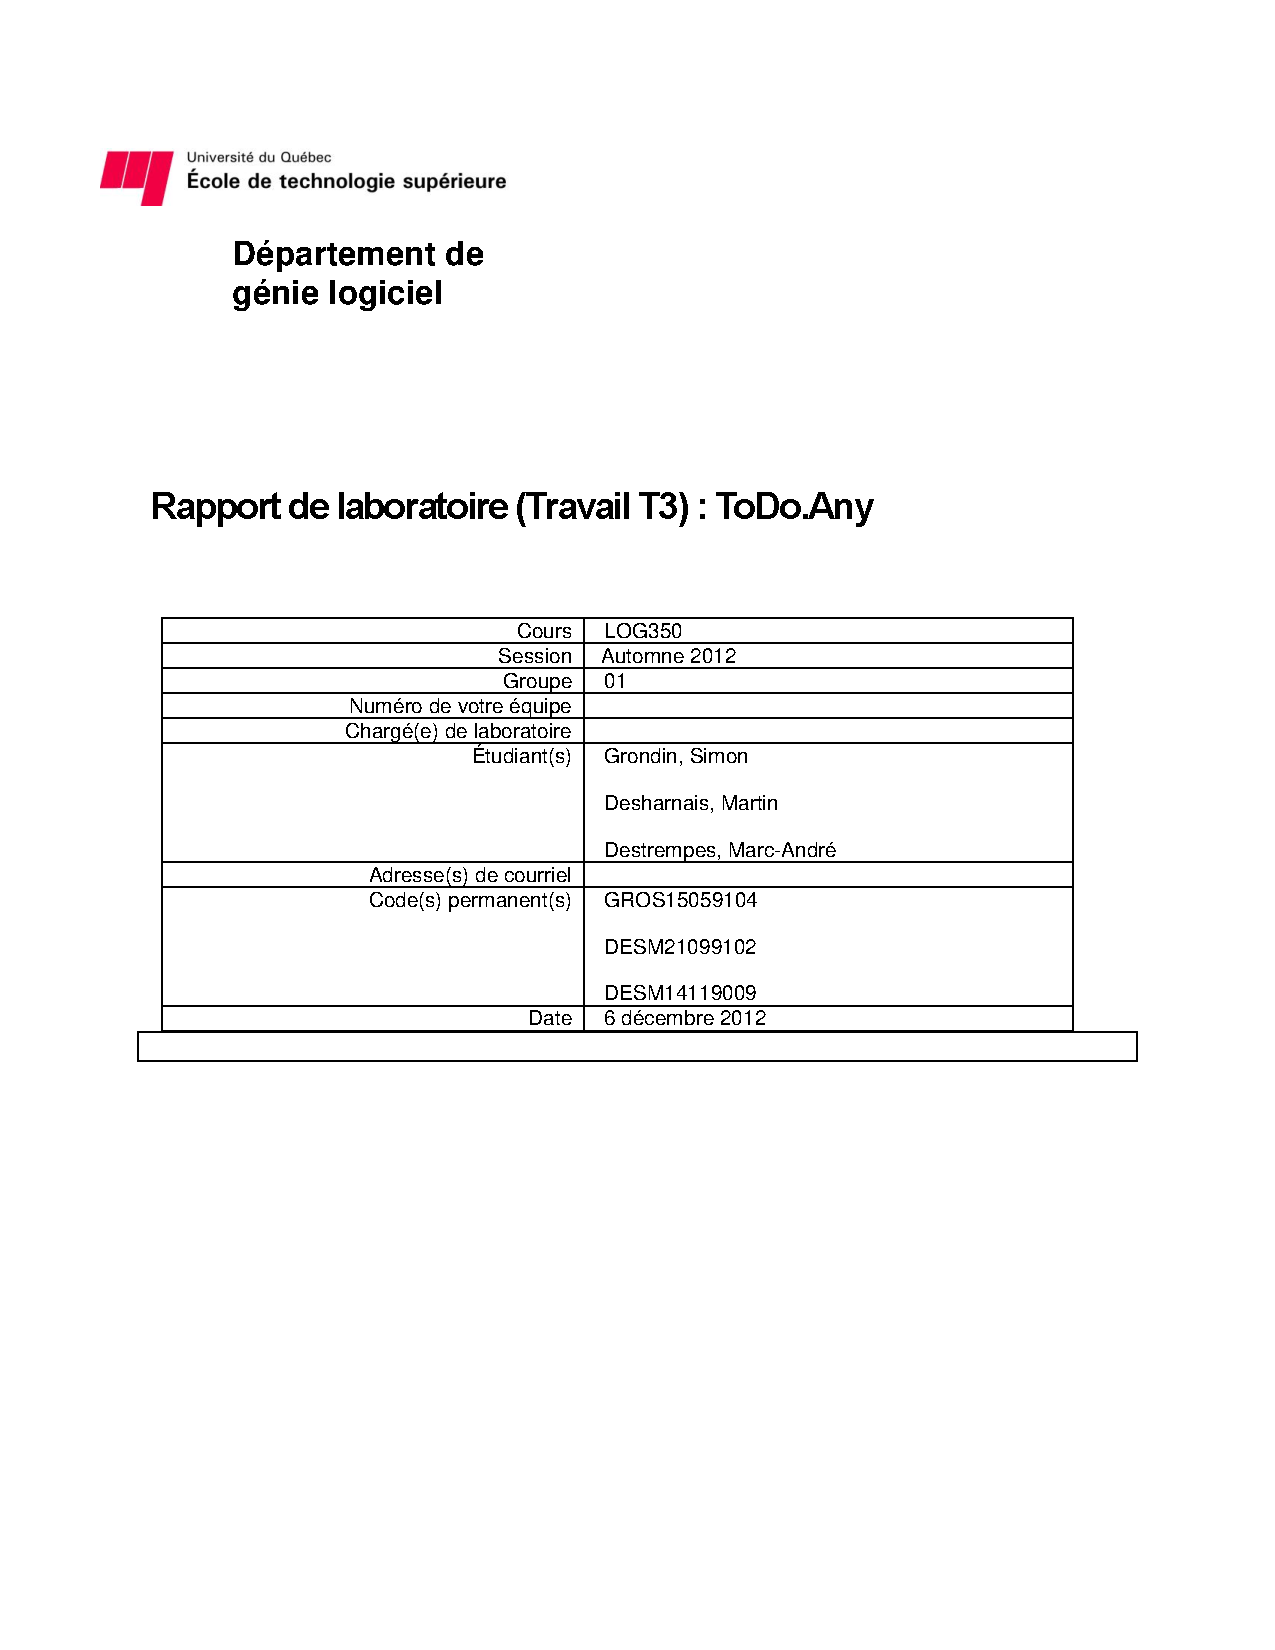
\includepdf[pages=-]{pageTitre.pdf}

\tableofcontents

%\listoftables
%\listoffigures

\frontmatter

\chapter{Glossaire}

\begin{description}
\item[C\#] est un langage de programmation orienté objet à typage fort, créé par la société Microsoft. \footnote{\url{https://fr.wikipedia.org/wiki/C_sharp}}
\item[Windows Presentation Foundation (WPF)] est la spécification graphique de Microsoft .NET 3.0. Il intègre le langage descriptif XAML qui permet de l'utiliser d'une manière proche d'une page HTML pour les développeurs. \footnote{\url{https://fr.wikipedia.org/wiki/Windows_Presentation_Foundation}}
\item[WinForms] est le nom de l'interface graphique qui est incluse dans .NET Framework, fournissant l'accès via du Managed code à l'API Windows. \footnote{\url{https://fr.wikipedia.org/wiki/Windows_Forms}}
\item[framework] est un kit de composants logiciels structurels, qui sert à créer les fondations ainsi que les grandes lignes de tout ou d’une partie d'un logiciel (architecture). \footnote{\url{https://fr.wikipedia.org/wiki/Framework}}
\item[.NET 4.5] est un framework pouvant être utilisé par un système d'exploitation Microsoft Windows et Microsoft Windows Mobile depuis la version 5 (.NET Compact Framework). \footnote{\url{https://fr.wikipedia.org/wiki/Framework_.NET}}
\item[SQLite] est une bibliothèque écrite en C qui propose un moteur de base de données relationnelle accessible par le langage SQL.\footnote{\url{https://fr.wikipedia.org/wiki/SQLite}}
\item[Git] est un logiciel de gestion de versions décentralisé. C'est un logiciel libre créé par Linus Torvalds, le créateur du noyau Linux, et distribué selon les termes de la licence publique générale GNU version 2.\footnote{\url{https://fr.wikipedia.org/wiki/Git}}
\item[DataGridView] est un élément graphique de type grille (table) qui est connecté directement sur la base de données.
\item[\LaTeX] est un langage et un système de composition de documents créé par Leslie Lamport en 1983. Plus exactement, il s'agit d'une collection de macro-commandes destinées à faciliter l'utilisation du « processeur de texte » TeX de Donald Knuth.\footnote{\url{https://fr.wikipedia.org/wiki/LaTeX}}
\end{description}

\mainmatter

\chapter{Introduction et sommaire du travail effectué en TP2}

L'application permet la gestion simple de tâches et d'événements tout en offrant des fonctionnalités de gestion et de classification avancées. Parmi celles-ci, notons la possibilite de définir des rappels, de catégoriser les éléments, de définir un événement comme échéance d'une tâche ou encore de définir des sous-tâches à une tâche imposante.

Durant notre analyse de tâches, nous avons déterminé que le public cible se compose de personnes de 15 ans et plus désirant organiser leur temps et leur vie professionnelle. De plus, nous avons conclu que notre interface devrait paraître familière et garder une courbe d'apprentissage faible. Pour se donner un point de départ, nous avons ainsi dressé une liste des cas d'utilisation que l'application doit traiter. Par la suite, nous avons construit nos prototypes statiques.

Nous avons utilisé des fenêtres virtuelles où chaque point de chaque fenêtre a été détaillé pour s'assurer que le travail devant être effectué par chaque interface a bel et bien été compris. De plus, chaque fonctionnalité a aussi été détaillée dans le but qu'elles soient bien comprisent.

Jusqu'à présent, presque aucune modification n'a été apportée entre les prototypes statiques et dynamiques sauf à quelques endroits pour des raisons de manque de temps et de personnel. Par exemple, dans la fenêtre Tâche, la section échéance a été changée. Pour le reste, tout va rester comme indiqué dans le document se trouvant à l'annexe III.

Dans le présent document, les tests qui seront effectués avec des utilisateurs sont listés et détaillés dans ce document. Par la suite, un concensus est fait pour chaque tâche et une amélioration possible est proposée pour améliorer le comportement du logiciel.

\chapter{Planification du travail}

\begin{table}
	\centering
	\begin{tabular}{|l|l|}
		\hline
		Semaine	& Travail accomplis 								\\ \hline \hline
		4 novembre	& Choix de la technologie et apprentissage de celle-ci.		\\ \hline
		11 novembre	& Marc-André : Conception des interfaces. 				\\
				& Martin : Conception de la base de données.				\\
				& Simon : Conception de la base de données.				\\ \hline
		18 novembre	& Marc-André : Début de la rédaction du rapport. 			\\ 
				& Martin : Programmation du prototype dynamique. 			\\
				& Simon : Programmation du prototype dynamique. 			\\ \hline
		25 novembre	& Marc-André : Rédaction du rapport.		 			\\
				& Martin : Programmation du prototype dynamique. 			\\ 
				& Simon : Programmation du prototype dynamique.		 	\\ \hline
		2 décembre	& Marc-André : Rencontre avec les utilisateurs. 			\\
				& Martin : Préparation de la présentation.				\\
				& Simon : Préparation de la présentation.				\\ \hline
		9 décembre	& Marc-André : Rédaction du rapport.	 				\\ 
				& Martin : Rédaction du rapport.	 					\\ 
				& Simon : Rédaction du rapport.			 			\\ \hline
	\end{tabular}
	\caption{Échéancier}
\end{table}

\chapter{Réalisation du prototype dynamique}

Dans la section suivante, nous vous présenterons notre prototype dynamique et donc, avant d'entreprendre la lecture de cette section, nous vous conseillons de lire le document se trouvant à l'annexe III. Ce document contient les informations concernant le prototype statique et toute la logique derrière le prototype dynamique.

\section{Choix des outils}

Pour réaliser le prototype dynamique, nous avons décidé d'utiliser le C\# et le Windows Presentation Foundation (WPF) comme langages de programmation. Nous avons choisi ces langages tout simplement parce que ceci nous permet de séparer le code des interfaces et que le WPF va nous permettre de créer des composantes et de les implémenter dans notre interface personnalisé plus facilement. 

Comme environnement de développement, nous utilisons Visual Studio 2012 avec le framework .NET 4.5 pour faciliter et accélérer notre développement. Ce framework nous donne des composantes graphiques de base qui nous simplifie la vie en nous permettant d'économiser du temps pour ne pas à avoir à developper des composants de base comme un TextBox ou un Label, par exemple.

De plus, comme base de données, nous utilisons SQLite parce que cela nous permet d'avoir un endroit pour stocker nos données de façon structuré et le tout dans un seul et unique fichier. Ce qui nous permet d'avoir une base de données portable.

Pour assurer la gestion des versions, nous utilisons un logiciel connu sous le nom de Git.

Pour la production de la documentation, nous utilisons le processeur de texte \LaTeX.

\newpage

\section{Fenêtres développées}

Dans cette section, chaque fenêtre de l'application est décrite brièvement et, par la suite, une justification est apportée pour différents choix de conception.

\subsection{Fenêtre principale}

Cette fenêtre comporte deux onglets offrant, pour le premier, une vue sur l'ensemble des événements et, pour le second, une vue sur l'ensemble des tâches. Le principe fondamental de l'application étant de permettre la gestion des tâches et des événements, cette fenêtre occupe la place centrale de l'interface utilisateur.

\begin{figure}
    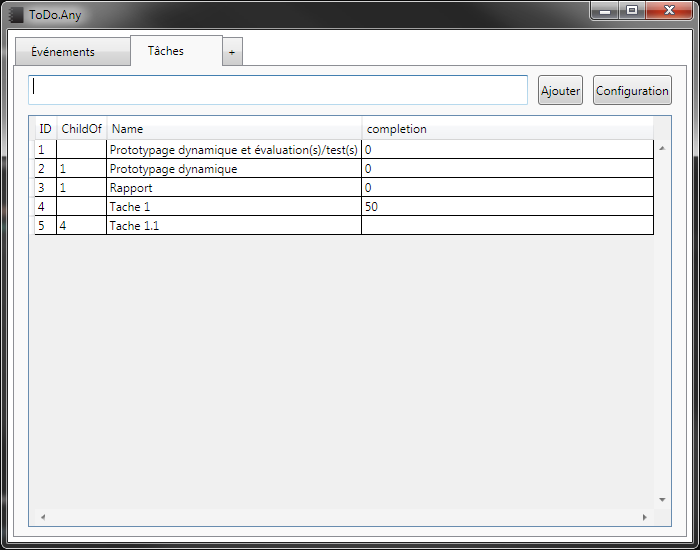
\includegraphics[scale=0.6]{fenetre_main.png}
    \caption{Fenêtre principale de l'application}
\end{figure}

Les onglets se présentent tous selon la même mise en page. Une barre comportant un champ texte et deux boutons se trouve dans la partie supérieure alors qu'une grille occupe l'espace restant. La grille permet d'afficher une liste d'éléments de façon hiérarchisée. Chaque ligne représente un élément et chaque colonne représente un champ d'information sur cet élément.

Lorsqu'un clic droit est fait sur une ligne de la grille, un menu contextuel apparait et offre la possibilité de supprimer l'élément concerné. De plus, double cliquer sur une ligne ouvrira une fenêtre apportant plus d'informations sur l'élément sélectionné.

La barre permet, quant à elle, d'ajouter un élément à la liste. Pour ce faire, il suffit d'entrer le nom du nouvel élément dans le champ texte et d'appuyer sur le bouton « Ajouter ». Le bouton « Configuration » permet, quant à lui, d'accéder aux configurations de l'application\footnote{à l'heure actuelle, la seule configuration possible est la gestion de la liste de priorités.}.

En plus des deux onglets permettant de visualiser l'ensemble des événements et l'ensemble des tâches, il est possible de créer de nouveaux onglets personnalisés à l'aide du bouton « + » prévu à cet effet. Un onglet personnalisé offre exactement les mêmes fonctionnalités qu'un onglet de base, mais offre en plus la possibilité de filtrer la liste d'éléments affichés selon leur respect de certains critères\footnote{En raison de contraintes de temps, nous n'avons malheureusement pas eu le temps d'implémenter cette fonctionnalité. Elle est présentée ici afin de bien saisir le fonctionnement de l'application, une fois celle-ci parfaitement fonctionnelle.}. Ainsi, il est possible de créer une liste n'affichant que les tâches concernant le travail ou bien encore une liste n'affichant que les tâches dont l'échéance se trouve dans les 48 prochaines heures.

Les critères utilisés pour filtrer la liste d'élément sont demandés lors de la création de la liste.

De plus, si une liste personnalisée n'est plus nécessaire, il est possible de la supprimer en cliquant sur le bouton « X » situé sur l'onglet correspondant.

\subsection{Événement}

Cette fenêtre contient les informations détaillées sur un événement. Elle est ouverte lorsque l'utilisateur double-clic sur une ligne de l'onglet « Événements ».

\begin{figure}
    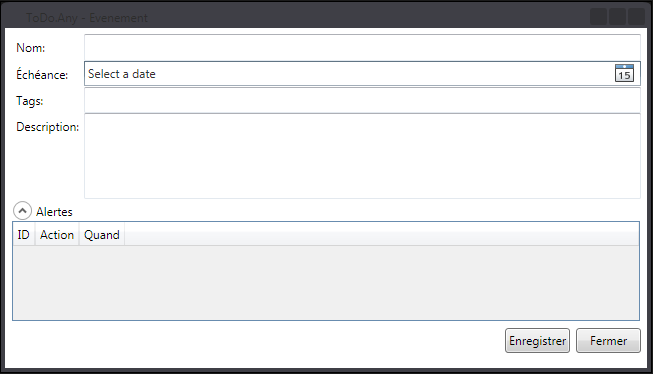
\includegraphics[scale=0.7]{fenetre_evenement.png}
    \caption{Fenêtre concernant un événement}
\end{figure}

Le nom est un texte identifiant un événement de façon unique (e.g. « Sortie à la ronde »). L'échéance est une date (e.g. « 2 juin 2013 ») et peut être entrée à l'aide d'un calendrier apparaissant lors d'un clic sur l'icône correspondante à droite. Les tags sont des informations permettant de catégoriser un événement (e.g. « [PERSONNEL][SORTIE] »). La description est un champ texte pouvant contenir plusieurs lignes et paragraphes.

La grille d'alertes permet d'entrer des actions (e.g « Envoyer un courriel ») qui devront être exécutées à un moment précis (e.g « 2 jours » avant la date d'échéance). Pour entrer une nouvelle alerte, il suffit d'entrer les informations dans la ligne vide. Un clic droit sur une ligne fera apparaître un menu contextuel permettant de supprimer l'alerte sélectionnée.

Lorsque l'une ou l'autre des informations est modifiée, le bouton « Enregistrer » est déverrouiller affin de permettre de sauvegarder les nouvelles informations. De plus, si la fenêtre est fermée alors qu'il y a des modifications en suspend, une boîte de dialogue demande s'il faut enregistrer avant de procéder à la fermeture de la fenêtre.

\subsection{Tâche}

Cette fenêtre contient les informations détaillées sur un événement. Elle est ouverte lorsque l'utilisateur double-clic sur une ligne de l'onglet « Événements ».

\begin{figure}
    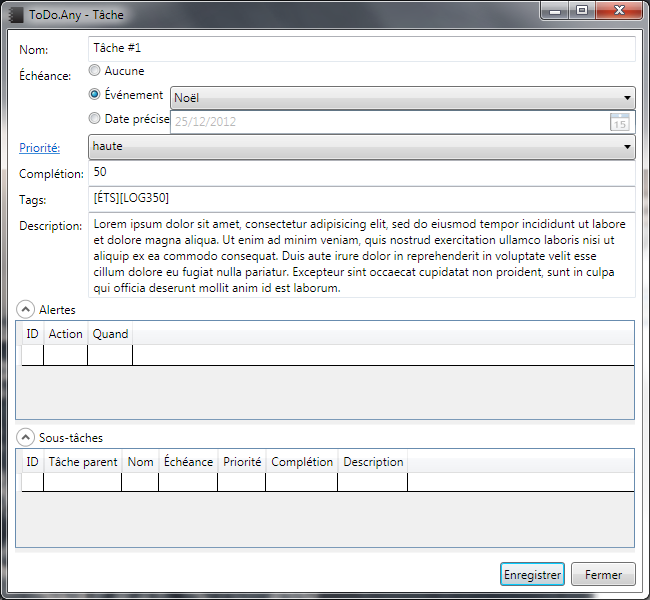
\includegraphics[scale=0.7]{fenetre_tache.png}
    \caption{Fenêtre concernant une tâche}
\end{figure}

Le nom est un texte identifiant une tâche de façon unique (e.g. « Faire le devoir de MAT265 »). L'échéance peut être un événement (e.g. doit être complété à l'événement « Examen final de MAT265 ») ou encore une date (e.g. doit être complété le « 14 décembre 2012 »). Dans le premier cas, l'événement peut être choisi dans une liste alors que, dans le deuxième cas, la date peut être entrée de la même manière que pour l'échéance d'un événement.

La priorité est un qualificatif permettant de spécifier qu'une tâche est plus importante qu'un autre et peut être choisie dans une liste. Si la priorité souhaitée ne se trouve pas dans la liste, il suffit de cliquer sur l'hyperlien « Priorité: » et la fenêtre permettant de configurer les priorités apparaitra.

La complétion est un pourcentage indiquant la proportion de la tâche qui est complétée. Les tags sont des informations permettant de catégoriser une tâche (e.g. « [ÉTS][MAT265] »). La description est un champ texte pouvant contenir plusieurs lignes et paragraphes.

La grille d'alerte fonctionne exactement de la même façon que pour un événement.

La grille de sous-tâches permet de séparer une tâche imposante en plusieurs tâches plus petites. Par exemple, la tâche « TP3 de LOG350 » peut être sous-divisée en deux sous-tâches : « Réalisation du prototype dynamique » et « Rédaction du rapport ». Pour créer une nouvelle tâche, il suffit d'entrer les informations dans la ligne vide. Un clic droit sur une ligne fera apparaître un menu contextuel permettant de supprimer la sous-tâche sélectionnée.

De plus, comme les sous-tâches sont des tâches à part entière. Il est possible d'ouvrir la fenêtre de détails d'une sous-tâche en double-cliquant sur la ligne désirée.

Lorsque l'une ou l'autre des informations est modifiée, le bouton « Enregistrer » est déverrouillé afin de permettre de sauvegarder les nouvelles informations. De plus, si la fenêtre est fermée alors qu'il y a des modifications en suspend, une boîte de dialogue demande s'il faut enregistrer avant de procéder à la fermeture de la fenêtre.

\subsection{Priorités}

Cette fenêtre permet de faire la gestion des priorités. Elle est ouverte à partir du bouton «·Configuration·» disponible dans chaque onglet de la fenêtre principale, ainsi qu'à partir de l'hyperlien « Priorité: » de la fenêtre de détails d'une tâche.

\begin{figure}
	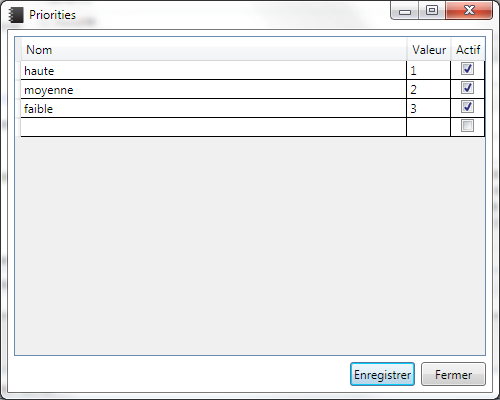
\includegraphics[scale=0.85]{fenetre_priorite.png}
	\caption{Fenêtre concernant les priorités}
\end{figure}

Le nom est un texte identifiant une priorité de façon unique. La valeur est un nombre donnant un poids aux différentes possibilités et permettant de les comparer entre elles. Ainsi, la priorité « Haute », qui a une la valeur un, est plus importante que la priorité « Faible », qui a la valeur trois.

L'attribut « Actif » indique s'il est possible3 d'utiliser cette priorité lors de la création de nouvelles tâches. Si l'attribut est coché, la priorité apparaitra dans la liste de priorité de la fenêtre de détails d'une tâche. Si l'attribut n'est pas coché, la priorité n'apparaîtra pas dans la liste, sauf si la tâche utilisait déjà la priorité lorsque celle-ci a été désactivée.

Lorsque l'une ou l'autre des informations est modifiée, le bouton « Enregistrer » est déverrouillé afin de permettre de sauvegarder les nouvelles informations. De plus, si la fenêtre est fermée alors qu'il y a des modifications en suspend, une boîte de dialogue demande s'il faut enregistrer avant de procéder à la fermeture de la fenêtre.

\newpage

\section{Justification des choix de conception}

Divers patrons de conception ont été utilisés pour parvenir à la conception de l'application que nous avons présentement. 

On compte entre autres le patron \emph{Many Workspaces} qui se retrouve à la fenêtre principale de l'application où l'utilisateur a la possibilité d'avoir plusieurs listes ouvertes et de les organiser comme il veut via les onglets.

\begin{figure}[H!]
	\centering
	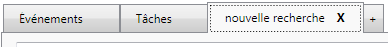
\includegraphics[width=1\textwidth]{many_workspaces.png}
	\caption{Onglets représentant différent espace de travail}
\end{figure}

Pour la navigation entre les fenêtres de l'application nous utilisons le patron \emph{Escape Hatch}. Ainsi, la navigation entre les fenêtres est limité et l'utilisateur peut toujours revenir a la fenêtre principale sans chercher pendant de longues minutes comment y revenir. Cela simplifie grandement l'interaction entre l'application et l'utilisateur en réduisant le processus de navigation au maximum.

\begin{figure}[H!]
	\centering
	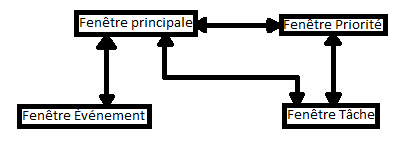
\includegraphics[width=1\textwidth]{navigation.png}
	\caption{Navigation entre les fenêtres}
\end{figure}

\newpage

Ensuite, pour ce qui est des listes, nous utilisons le patron \emph{Tree Table} sur, par exemple, la fenêtre principale. Avec ce patron, nous listons donc les tâches et ses sous-tâches sous la tâche correspondante sous forme d'arborescence. Nous pouvons donc afficher un maximum d'information utile à l'utilisateur lorsque celui-ci le demande. Par manque de temps et de ressources humaines, ce patron a été implanté partiellement.

\begin{figure}[H!]
	\centering
	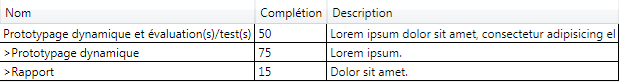
\includegraphics[width=1\textwidth]{tree_table.png}
	\caption{DataGridView avec le patron \emph{Tree Table}}
\end{figure}

Nous utilisons aussi le patron \emph{New-Item Row} dans la fenêtre Priorités, par exemple, pour permettre l'ajout rapide et infini de lignes dans le tableau sans que l'utilisateur n'ait besoin d'appuyer sur quoi que se soit. 

\begin{figure}[H!]
	\centering
	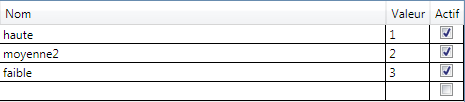
\includegraphics[width=1\textwidth]{new_item_row.png}
	\caption{DataGridView avec le patron \emph{New-Item Row}}
\end{figure}

Pour ce qui est de toutes les grilles, le patron \emph{Sortable Table} s'applique et permet de trier l'information affichée en tout temps pour permettre à l'utilisateur de trouver ce qu'il veut plus rapidement.

\begin{figure}[H!]
	\centering
	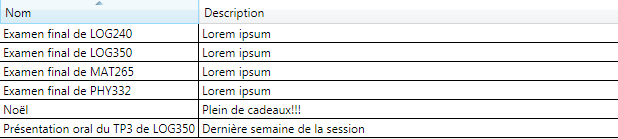
\includegraphics[width=1\textwidth]{sortable_table.png}
	\caption{Exemple d'une colonne trié}
\end{figure}

De plus, nous avons respecté le plus possible le contenu de la norme \emph{ISO 9241-120} à \emph{ISO 9241-129} qui traite sur les interactions sur les entrées, les sorties et les interactions.

Quelques changements on été effectués entre les prototypes statique et dynamique. Parmi ces changements, on compte les options possibles pour une échéance dans la fenêtre sur les tâches. Ce changement a été fait dû aux limitations logicielles et par faute de temps. Il est à noter que ces changements n'influencent en aucun cas l'efficacité de l'application.

\section{Améliorations possibles}

Quelques améliorations possibles seraient d'utiliser les lois psychomotrices de Fitts et Miller pour optimiser l'interface. Nous pourrions ainsi optimiser les déplacements que l'utilisateur doit faire avec sa souris pour cliquer sur les boutons et les champs de saisies dans les fenêtres. Par faute de temps et de ressources humaines, il nous est donc impossible d'effectuer ces tests.

\chapter{Démonstration du prototype dynamique en laboratoire}

Un prototype dynamique de l'application est disponible à l'adresse suivante : \\
\url{https://github.com/xeph/LOG350.TP3}.

Évaluation du prototype en laboratoire  : le 4 décembre 2012 au laboratoire (pour les 2 groupes).

Exposé oral  : le 6 décembre 2012 dans un local à définir (pour les 2 groupes).

Remise du code final : le 11 décembre 2012 à 23h59 maximum par courriel à log350a2012@gmail.com.

Remise du rapport :  le 11 décembre 2012 à 23h59 maximum en version papier dans la chute du département.

Remise de la présentation de l’exposé oral : le 6 décembre 2012 à 23h59 maximum par courriel à log350a2012@gmail.com.

\chapter{Tests avec utilisateurs}

\section{Méthodologie}

Avant d'effectuer les tests, un document expliquant la nature du projet et le déroulement des tests a été fourni aux utilisateurs. Les membres de l'équipe assument que le document a été lu lors de la rencontre. De plus, un formulaire de consentement sera obligatoirement signé par l'utilisateur et un membre de l'équipe pour que les deux parties s'entendent sur ce qui sera fait lors de la rencontre.

Pour faire les tests avec les utilisateurs, le ou les membres de l'équipe s'asseoiront avec l'utilisateur qui testera l'application. Par la suite, un membre de l'équipe se chargera de dire chaque tâche que l'utilisateur devra effectuer et si l'utilisateur a des questions, il sera chargé de lui fournir les informations. Lorsque l'utilisateur aura terminé de faire une tâche, il y aura une brève pause pour que tout le monde ait le temps de prendre des notes. L'exécution de la tâche suivante se fera lorsque tout le monde aura terminé de prendre les notes pour la tâche courante. Quand toutes les tâches auront été exécutées, l'utilisateur pourra donner son opinion et ses impressions sur l'application, suggérer améliorations, les points positifs et des fonctionnalitées qui pourraient être intéressantes à ajouter ou bien améliorer.

Ce seront principalement des notes concernant la performance et l'usabilité de l'application qui seront prises, car les principaux objectifs que nous voulons atteindre avec notre application sont 1- la facilité d'utilisation et 2- l'efficacité. Les notes seront tirées de l'interaction de l'utilisateur avec l'application et de la rapidité avec laquelle l'utilisateur effectue les tâches (l'efficacité).

Les tests se feront dans le calme et le respect. De plus, l'utilisateur peut, en tout temps, décider d'arrêter les tests sans devoir fournir une explication. Les données recueillies seront cependant conservées à moins que l'utilisateur ne demande à ce qu'elles soient détruites.

\newpage

\section{Liste des tâches}

\bottomcaption{Liste des tâches}
\begin{supertabular}{|p{1cm}|p{7.5cm}|p{6cm}|}
    \hline
    No tâche & Titre et description & Éléments à vérifier et hypothèses \\ \hline \hline
    1 & Ajouter l'événement « événement 1 ». & Détection de raccourcis. \\ \hline
    2 & Définir l’échéance de « événement 1 » au 1 janvier 2013. & \\ \hline
    3 & Ajouter le tag « [TAG1] » à « événement 1 ». & \\ \hline
    4 & Ajouter une alerte « Envoyer un courriel », « 2 », « jours ». & \\ \hline
    5 & Enregistrer l’événement. & \\ \hline
    6 & Fermer la fenêtre. & \\ \hline
    7 & Supprimer l’événement « Examen final de PHY332 ». & Détection de menu contextuel. \\ \hline
    8 & Ajouter la tâche « tâche 1 ». & Détection de raccourcis. \\ \hline
    9 & Définir l’échéance de « tâche 1 » comme étant l’événement « événement 1 ». & \\ \hline
    10 & Définir la priorité de  « tâche 1 » à « Très faible ». <NE PEUT PAS ÊTRE FAIT> & Détection de raccourcis. \\ \hline
    11 & Ajouter la priorité « très faible » avec une valeur de « 4 » et Actif à « Vrai » et enregistrer. & \\ \hline
    12 & Définir la priorité de  « tâche 1 » à « Très faible ». & L'utilisateur s'attent-il que la liste de prioritées ait été automatiquement actualisée? \\ \hline
    13 & Définir la complétion de « tâche 1 » à « 42 ». & \\ \hline
    14 & Ajouter les tags « [TAG1] » et « [TAG2] » à « tâche 1 ». & \\ \hline
    15 & Ajouter la description « lorem ipsum » à « tâche 1 ». & \\ \hline
    16 & Ajouter une alerte « afficher un rappel », « 5 », « minutes » à « tâche 1 ». & \\ \hline
    17 & Créer une sous-tâche « tâche 1.1 » à « tâche 1 ». & \\ \hline
    18 & Créer une sous-tâche « tâche 1.2 » à « tâche 1 ». & \\ \hline
    19 & Enregistrer la tâche. & \\ \hline
    20 & Fermer la fenêtre. & \\ \hline
    21 & Supprimer la « tâche 1.2 » & \\ \hline
    22 & Modifier l’échéance de « tâche 1 » pour le « 3 février 2013 ». & \\ \hline
    23 & Fermer la fenêtre. & L'utilisateur a-t-il pensé qu'il devait enregistrer? \\ \hline
    24 & Appuyer sur « Annuler ». & \\ \hline
    25 & Définir la complétion de la « tâche 1 » à « 50 ». & \\ \hline
    26 & Fermer la fenêtre. & \\ \hline
    27 & Appuyer sur « Oui ». & \\ \hline
    28 & Appuyer sur le bouton « Configuration ». & \\ \hline
    29 & Définir la priorité « très faible » à « non-actif » & \\ \hline
    30 & Fermer la fenêtre. & \\ \hline
    31 & Appuyer sur « Oui ». & \\ \hline
    32 & Modifier la priorité de la « tâche 1 » à « faible ». & L'utilisateur se remarque-t-il que la tâche est toujours valide même si sa prioritée vient d'être désactivée? \\ \hline
    33 & Enregistrer la tâche. & \\ \hline
    34 & Fermer la fenêtre. & \\ \hline
\end{supertabular}

\section{Liste des utilisateurs}

Les caractéristiques principales des utilisateurs choisis sont la gestion de leurs tâches pour les travaux et devoirs au CÉGEP ou bien à l'université et la gestion des rendez-vous pour les professionnels. Nous avons choisis ce nombre d'utilisateurs, car il nous fallait un petit échantillon oeuvrant dans le même type de vie que le public visé, mais dans des sphères professionnelles différentes.

\newpage

\section{Résultats}

\begin{table}
	\centering
	\begin{tabular}{|l|l|l|}
	\hline
	no Tâche	& Points importants de l'observation	\\ \hline \hline
	1		& a ajouté une ligne vide et double	\\ 
			& cliquer sur l'entrée ensuite		\\ \hline
	2		& 						\\ \hline
	3		& 						\\ \hline
	4		& a pesé sur	$\bigtriangleup$ en $1^{er}$ \\
			& n'entre pas le 2 (date à la place)	\\ \hline
	5		& 						\\ \hline
	6		& 						\\ \hline
	7		& ne trouve pas coment supprimer	\\ \hline
	8		& n'utilise pas la barre d'ajout rapide	\\ \hline
	9		& 						\\ \hline
	10		& 						\\ \hline
	11		& 						\\ \hline
	12		& 						\\ \hline
	13		& 						\\ \hline
	14		& ; au lieu de les coller			\\ \hline
	15		& 						\\ \hline
	16		& 						\\ \hline
	17		& 						\\ \hline
	18		& 						\\ \hline
	19		& 						\\ \hline
	20		& 						\\ \hline
	21		& 						\\ \hline
	22		& 						\\ \hline
	23		& 						\\ \hline
	24		& 						\\ \hline
	25		& 						\\ \hline
	26		& 						\\ \hline
	27		& 						\\ \hline
	28		& 						\\ \hline
	29		& 						\\ \hline
	30		& 						\\ \hline
	31		& 						\\ \hline
	32		& 						\\ \hline
	33		& 						\\ \hline
	34		& 						\\ \hline
	\end{tabular}
	\caption{Résultats de l'utilisateur 1}
\end{table}

\newpage

\begin{table}
	\centering
	\begin{tabular}{|l|l|l|}
	\hline
	no Tâche	& Points importants de l'observation	\\ \hline \hline
	1		& n'utilise pas la barre d'ajout rapide	\\ \hline
	2		& 						\\ \hline
	3		& 						\\ \hline
	4		& a pesé sur	$\bigtriangleup$ en $1^{er}$ \\ \hline
	5		& 						\\ \hline
	6		& 						\\ \hline
	7		& ne trouve pas coment supprimer	\\ \hline
	8		& ne trouve pas tâche			\\ \hline
	9		& 						\\ \hline
	10		& 						\\ \hline
	11		& 						\\ \hline
	12		& 						\\ \hline
	13		& 						\\ \hline
	14		& 						\\ \hline
	15		& 						\\ \hline
	16		& 						\\ \hline
	17		& 						\\ \hline
	18		& 						\\ \hline
	19		& 						\\ \hline
	20		& 						\\ \hline
	21		& 						\\ \hline
	22		& 						\\ \hline
	23		& 						\\ \hline
	24		& 						\\ \hline
	25		& 						\\ \hline
	26		& 						\\ \hline
	27		& 						\\ \hline
	28		& 						\\ \hline
	29		& changer le nom au lieu du check box	\\ \hline
	30		& 						\\ \hline
	31		& 						\\ \hline
	32		& 						\\ \hline
	33		& 						\\ \hline
	34		& 						\\ \hline
	\end{tabular}
	\caption{Résultats de l'utilisateur 2}
\end{table}

\newpage

\section{Discussion et recommandations}

\begin{table}
	\centering
	\begin{tabular}{|l|l|l|}
	\hline
	no Tâche	& Résumé	& Recommandation 	\\ \hline \hline
	1		&  n'utilise pas la barre d'ajout rapide		&  mettre la barre plus visible			\\ \hline
	2		& 							&  							\\ \hline
	3		& 							&  							\\ \hline
	4		& a pesé sur $\bigtriangleup$ en $1^{er}$	& donner plus d'informations sur les expander \\ \hline
	5		& 							&  							\\ \hline
	6		& 							&				  			\\ \hline
	7		& ne trouve pas coment supprimer		&  fournir un bouton supprimer			\\ \hline
	8		& 							&  							\\ \hline
	9		& 							&  							\\ \hline
	10		& 							&  							\\ \hline
	11		& 							&  							\\ \hline
	12		& 							&  							\\ \hline
	13		& 							&  							\\ \hline
	14		& 							&  							\\ \hline
	15		& 							&  							\\ \hline
	16		&							&  							\\ \hline
	17		& 							&  							\\ \hline
	18		& 							&  							\\ \hline
	19		& 							&  							\\ \hline
	20		& 							&  							\\ \hline
	21		& 							&  							\\ \hline
	22		& 							&  							\\ \hline
	23		& 							&  							\\ \hline
	24		& 							&  							\\ \hline
	25		& 							&  							\\ \hline
	26		& 							&  							\\ \hline
	27		& 							&  							\\ \hline
	28		& 							&  							\\ \hline
	29		& 							&  							\\ \hline
	30		& 							&  							\\ \hline
	31		& 							&  							\\ \hline
	32		& 							&  							\\ \hline
	33		& 							&  							\\ \hline
	34		& 							&  							\\ \hline
	\end{tabular}
	\caption{Recommandations par les observateurs}
\end{table}

\newpage

\begin{table}
	\centering
	\begin{tabular}{|l|l|l|}
	\hline
	no Tâche	& Résumé	& Recommandation 	\\ \hline \hline
	1		&  n'utilise pas la barre d'ajout rapide		&  modifier la barre d'ajout \\ \hline
	2		& 							&  									\\ \hline
	3		& 							&  									\\ \hline
	4		& a pesé sur $\bigtriangleup$ en $1^{er}$	& donner plus d'information sur les expander \\ \hline
	5		& 							&  									\\ \hline
	6		& 							&  									\\ \hline
	7		& ne trouve pas coment supprimer		&  changer l'endroit ou se trouve supprimer			\\ \hline
	8		& 							&  									\\ \hline
	9		& 							&  									\\ \hline
	10		& 							&  									\\ \hline
	11		& 							&  									\\ \hline
	12		& 							&  									\\ \hline
	13		& 							&  									\\ \hline
	14		& 							&  									\\ \hline
	15		& 							&  									\\ \hline
	16		&							&  									\\ \hline
	17		& 							&  									\\ \hline
	18		& 							&  									\\ \hline
	19		& 							&  									\\ \hline
	20		& 							&  									\\ \hline
	21		& 							&  									\\ \hline
	22		& 							&  									\\ \hline
	23		& 							&  									\\ \hline
	24		& 							&  									\\ \hline
	25		& 							&  									\\ \hline
	26		& 							&  									\\ \hline
	27		& 							&  									\\ \hline
	28		& 							&  									\\ \hline
	29		& 							&  									\\ \hline
	30		& 							&  									\\ \hline
	31		& 							&  									\\ \hline
	32		& 							&  									\\ \hline
	33		& 							&  									\\ \hline
	34		& 							&  									\\ \hline
	\end{tabular}
	\caption{Recommandations par les utilisateurs}
\end{table}

La barre d'ajout rapide plante dans un nouvel onglet (SearchTasks.xaml.cs), les bugs n'ont pu être reproduits.

\chapter{Changements recommandés}

À la suite des tests avec les utilisateurs, nous avons établi une liste de modifications recommandées afin de rendre l'interface utilisateur plus simple et plus efficace.

\section{Améliorer la barre d'ajout rapide}

Nous avons observé deux faits étonnants concernant la fenêtre principale : la fonctionnalité d'ajout rapide n'a pas été utilisée et les utilisateurs croyaient que le champ texte servait à rechercher un élément dans la grille. Ceci nous amène à revoir le concept de la barre d'ajout rapide.

Après quelques réflexions et discussions avec les utilisateurs, nous avons décidé qu'il serait mieux de revoir la fonction du champ texte, situé en haut des listes de tâche et d'événements, et le transformer en barre de recherche et d'ajout. Ainsi, lorsque du texte sera tapé à l'intérieur, la grille au-dessous sera automatiquement actualisée pour ne contenir que les éléments dont le nom contenant le texte entré. Ceci permettra donc de retrouver plus rapidement un élément précis lorsque la grille sera pleine.

De plus, dès que l'utilisateur commencera à entrer du texte, une bulle contenant le texte « Créer un nouvel élément portant le nom ... » apparaitra sous la barre. Si l'utilisateur appui sur le bouton « entrer » ou clique sur le texte, un nouvel élément sera créé, ajouté à la liste et la barre sera vidée de son texte. Comme l'option d'ajouter une nouvelle tâche n'apparait que lorsque nécessaire, nous allons enlever le bouton « Ajouter » qui serait redondant.

Ce comportement n'est pas sans rappeler la barre de navigation du logiciel Google Chrome qui, lorsque l'utilisateur commencer à y entrer du texte, lance une recherche dans l'historique de navigation, en affiche les résultats et offre la possibilité de lancer une recherche Google.

\begin{figure}
    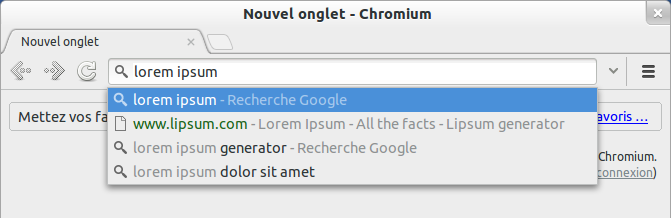
\includegraphics[scale=0.5]{barre_de_navigation_google_chrome.png}
    \caption{Barre de navigation de Google Chrome}
\end{figure}

\section{Simplifier le champ complétion}

Nous avons aussi remarqué que les utilisateurs n'étaient pas certains de ce qu'ils devaient entrer dans le champ « Complétion » de la fenêtre « Tâche ». Est-ce un qualificatif, un pourcentage ou bien un nombre quelconque?

Pour remédier à cette incertitude, nous avons décidé de remplacer le champ texte actuellement présent par un curseur de défilement (mieux connu sous le nom « slider », en anglais). Celui-ci aura la double responsabilité de rendre plus explicite le fait que la complétion est un pourcentage, s'assurera qu'il est impossible d'entrer une valeur erronée et sera beaucoup plus facile d'utilisation.

Pour entrer un niveau de complétion, l'utilisateur pourra simplement glisser le curseur jusqu'à ce que le pourcentage affiché corresponde à la valeur recherchée. D'un autre coté, il aura aussi le choix de garder les mains sur le clavier en utilisant les flèches du clavier pour faire glisser le curseur vers la droite ou la gauche.

Une possibilité supplémentaire qui mérite d'être étudiée est de verrouiller le contrôle et calculer automatiquement le niveau de complétion lorsqu'une tâche à des sous-tâches qui ont elles-mêmes un niveau de complétion. Ainsi, une tâche ayant deux sous-tâches, une complétée à 100 pour cent et l'autre complétée à 50 pour cent, pourrait se faire assigner automatiquement un niveau de complétion de 75 pour cent.

\begin{figure}
    
\includegraphics[scale=0.25]{completion2.png}
    \caption{Slider de complétion}
\end{figure}

\section{Simplifier la barre de tags}

Les utilisateurs ont unanimement affirmé que la façon dont les tags sont actuellement entrés est trop compliquée et sujette à erreurs. Pour rappel, le format actuel est complètement textuel. Un tag est une suite de caractères entourée de crochets et il est possible d'entrer plusieurs tags les plaçant les uns à la suite des autres (e.g. « [ÉTS][LOG350][TP3] »).

Pour faciliter l'entrée de tags, nous avons décidé qu'il serait plus efficace de se baser sur le système d'entrée de tags du site StackOverflow. Le principe est que le champ contenant n'est pas un simple champ texte, mais une liste de tags qu'il est possible de manipuler avec la souris. Ainsi, chaque tag a un petit « x » qui permet de l'enlever de la liste et la liste peut être réordonnée en glissant \& déposant les tags les uns à côté des autres.

Cependant, c'est lors de l'ajout d'un nouveau tag que la différence est la plus flagrante. Lorsque l'utilisateur commencera à entrer du texte, une fenêtre apparaîtra et offrira une liste de suggestions basées sur les tags déjà présents dans les autres tâches. L'utilisateur pourra alors cliquer sur le tag de son choix pour le sélectionner. De plus, le premier élément de la liste sera surligné par défaut et sera choisi automatiquement si l'utilisateur appuie sur la touche « entrer ».

Enfin, si l'utilisateur veut entrer un nouveau tag qui n'apparait pas dans la liste, il suffira d'appuyer sur la barre d'espacement et le nouveau tag sera ajouté à la liste.

\begin{figure}
    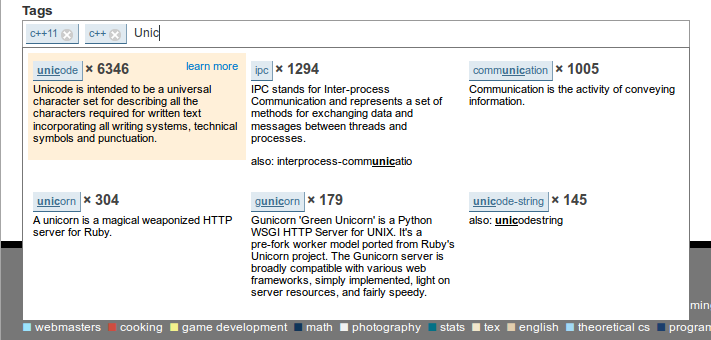
\includegraphics[scale=0.5]{tags_stackoverflow.png}
    \caption{Barre de tags du site www.stackoverflow.com}
\end{figure}

\section{Ajouter des infobulles}

Lorsque nous avons présenté notre application à différents utilisateurs, nous avons occasionnellement eu à répondre à des questions telles que :

\begin{itemize}
    \item Qu'est-ce qu'une échéance?
    \item Qu'est-ce qu'un tag?
    \item À quoi sert une alerte?
\end{itemize}

Comme nous nous trouvions juste à côté des utilisateurs, il était facile pour nous de leur donner des explications. Seulement, s'ils avaient été seuls, il aurait pu être difficile pour eux d'obtenir des réponses à leurs questions.

Pour tenter de minimiser la courbe d'apprentissage et d'améliorer la compréhension des utilisateurs, nous avons décidé de placer des infobulles expliquant les différentes informations qu'ils peuvent entrer et les différentes actions qu'ils peuvent poser.

Par exemple, le concept de tag peut sembler étrange à quelqu'un qui n'a jamais été confronté à ce concept. Aussi, le fait qu'un événement puisse être considéré comme l'échéance d'une tâche peut ne pas sembler évident au premier abord.

Les infobulles ne serviront donc pas seulement pour les boutons ne comportant pas de texte, mais aussi pour offrir une explication pour la signification de certains composants.

\begin{figure}
    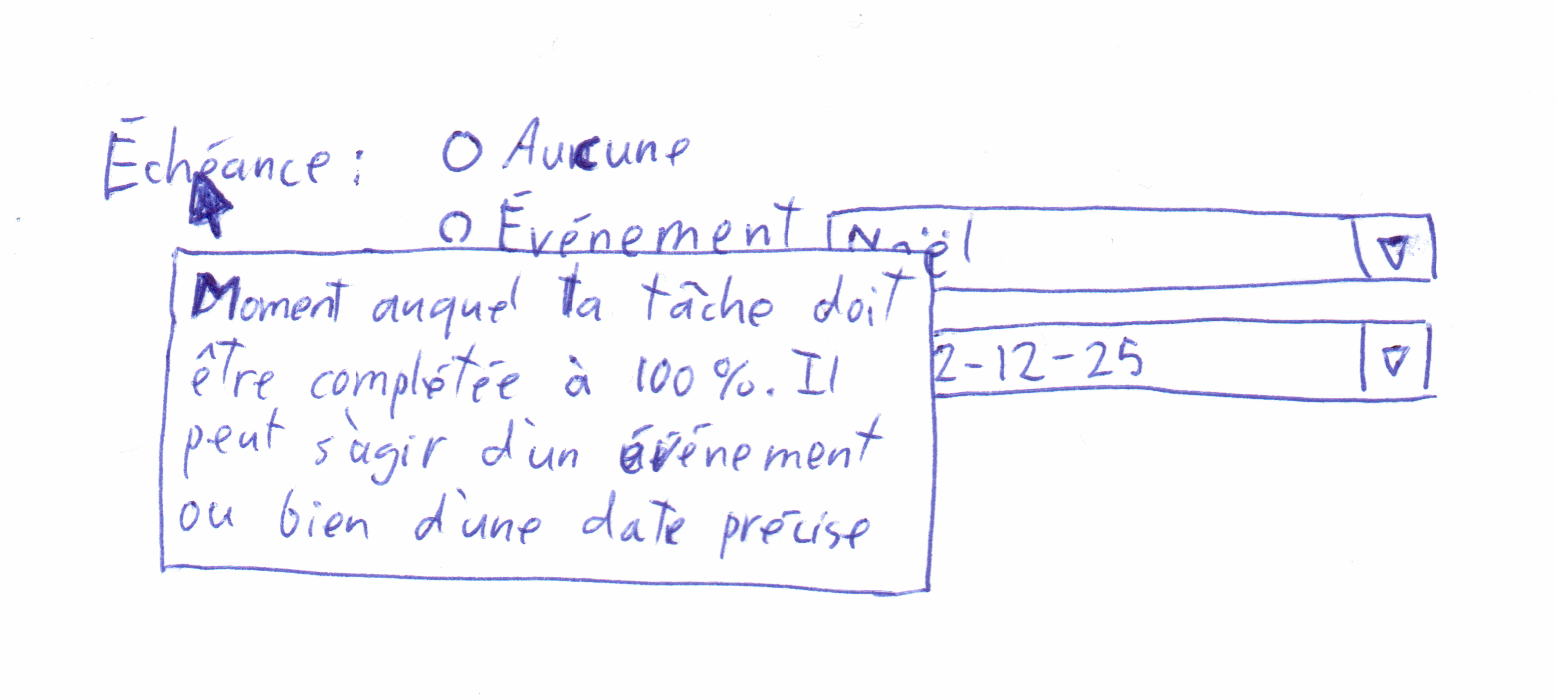
\includegraphics[scale=0.2]{infobulle.png}
    \caption{Infobulle expliquant le concept d'échéance}
\end{figure}

\section{Ajouter le support du glisser \& déposer}

L'objectif principal de la fenêtre d'ajout rapide est de permettre de faire une gestion simple de ses tâches sans avoir à entrer dans la fenêtre de détails d'une tâche. Seulement, s'il est actuellement possible de créer autant de tâches que l'on veut à partir de la fenêtre principale, il est nécessaire d'ouvrir la fenêtre de détails afin de pouvoir créer des sous-tâches.

La méthode que nous avons choisie pour remédier à cette situation est d'ajouter le support du glisser \& déposer dans la grille de la fenêtre principale. L'objectif est de pouvoir modifier la structure de tâches parent-enfant en glissant les tâches les unes sur les autres.

Ainsi, pour créer la tâche du laboratoire 3 de LOG350, il suffira de :

\begin{enumerate}
    \item Entrer « Laboratoire 3 de LOG350 » dans la barre d'ajout.
    \item Appuyer sur la touche « entrer ».
    \item Entrer « Réaliser le prototype dynamique » dans la barre d'ajout.
    \item Appuyer sur la touche « entrer ».
    \item Sélectionner la tâche « Réaliser le prototype dynamique » et la glisser sur la tâche « Laboratoire 3 de LOG350 ».
    \item Entrer « Rédaction du rapport » dans la barre d'ajout.
    \item Appuyer sur la touche « entrer ».
    \item Sélectionner la tâche « Rédaction du rapport » et la glisser sur la tâche « Laboratoire 3 de LOG350 ».
\end{enumerate}

\chapter{Conclusion}

En conclusion, ce projet a été l'occasion de faire une incartade dans le monde du développement d'interfaces utilisateurs. Nous avons eu l'occasion de participer et d'en apprendre plus sur les différentes étapes de conception : analyse de tâches, prototype statique et prototype dynamique.

D'abord, l'analyse de tâches et le prototype statique nous ont amené à comprendre l'importance de bien connaître son public afin de produire des interfaces utilisateurs qui correspondent réellement à ses besoins. Pour ce faire, nous avons utilisé le vieux principe d'être notre propre public cible. Nous nous sommes demandé quels sont les besoins que nous avions pour gérer notre emploi du temps efficacement et avons tenté de concevoir un système qui réponde à ces exigences. Nous sommes partis du principe que, si nous arrivions à produire un logiciel qui réponde à nos propres besoins, le projet pourrait être considéré comme une réussite.

Par la suite, nous nous sommes demandé si une telle application pouvait être utile à un auditoire plus élargi. Nous avons présenté notre concept et nos idées à des personnes tierces et avons recueilli leurs commentaires et réactions afin de peaufiner quelques détails. Cette expérience nous a confortés dans notre idée que, si des concepteurs connaissent bien leurs utilisateurs et arrivent à penser comme eux, le système produit est plus adapté et plus cohérent.

Ensuite, la réalisation du prototype dynamique nous a appris l'importance, pour un développeur, de bien connaître ses outils avant de s'engager dans la conception d'un système. Au début du projet, nous avons décidé d'utiliser la bibliothèque graphique WPF, une technologie nouvelle pour nous, et nous sommes dit que nous l'apprendrions au fil de l'avancement du projet. Ceci s'est avéré plus difficile que prévu.

Il s'est d'abord avéré assez rapide et facile de faire fonctionner une interface simple utilisant les composants fournis de base. Malheureusement, la situation s'est complexifiée lorsque nous avons voulu implémenter des interfaces nécessitant des composants qui n'existent pas dans la bibliothèque. Toutes les briques nécessaires pour construire de tels composants sont disponibles, mais acquérir les compétences pour développer de nouveaux contrôles WPF prend beaucoup plus de temps que ce que nous avions à notre disposition.

Le meilleur exemple de ces difficultés rencontrées est le système multionglets. Dans la phase d'analyse et de réalisation du prototype statique, nous avions l'intention d'offrir la possibilité de définir des vues plus spécialisées de la liste de tâches dans des onglets supplémentaires. Il aurait alors été possible de créer une vue qui n'affiche que les tâches concernant l'université ou bien uniquement les tâches qui doivent être complétées dans les 48 prochaines heures. Malheureusement, il a fallu tellement de temps pour réussir à implémenter un contrôle permettant à l'utilisateur de créer et supprimer des onglets que nous n'avons pas eu le temps et les ressources nécessaires pour implémenter la fonctionnalité de requête pour configurer une vue.

Enfin, il est ressorti de nos différentes conversations avec des utilisateurs que plusieurs trouvaient l'application visuellement « ordinaire », mais qu'aucun n'avait la même opinion de ce qui permettrait de la rendre plus « belle ». Parmi les membres de notre équipe, aucun ne se considère comme un artiste et ne sait comment créer un arrangement de formes et de couleurs qui plairait à une majorité. Cette constatation met de l'avant le fait qu'il y a une différence importante entre développer une interface efficace et une interface visuellement attirante. Le cours que nous avons suivi tente de nous apprendre à développer la première, mais ne prétend nullement nous apprendre à développer la seconde.

Concernant le cours, nous suggérons que celui-ci donne une plus grande place aux applications dites de bureau. Celles-ci étant encore très présentes comme applications « grand public » et largement dominantes dans le monde professionnel, il serait intéressant qu'elles occupent une plus grande place. Certaines sont très simples d'utilisation alors que d'autres sont incroyablement complexes. Qu'est-ce qui les distingue? Quelles sont les bonnes habitudes à imiter? Quelles sont les erreurs à ne pas commettre?

\appendix
\multiannexe

\chapter{Document de présentation du projet}

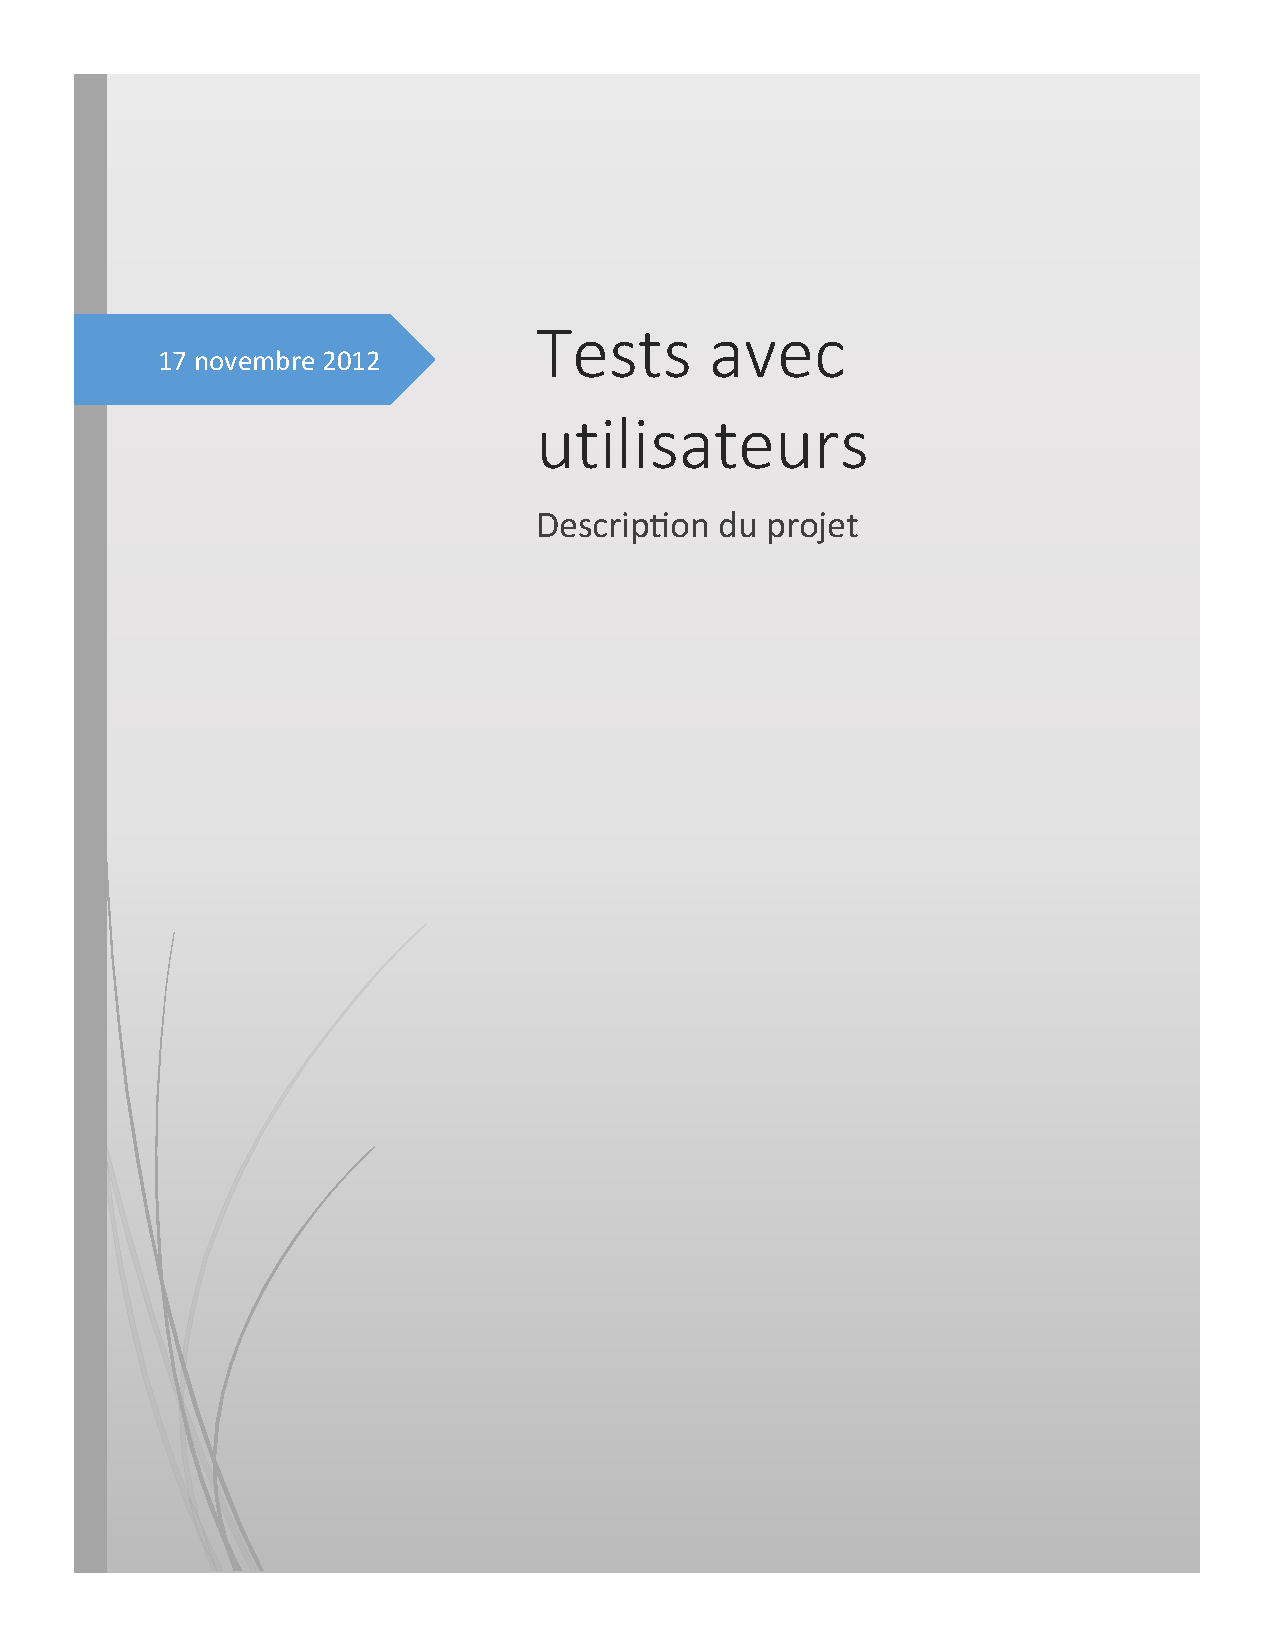
\includepdf[pages=-]{document.pdf}

\chapter{Formulaires de consentement signés}

%
\includepdf[pages=-]{form_u0.pdf}
%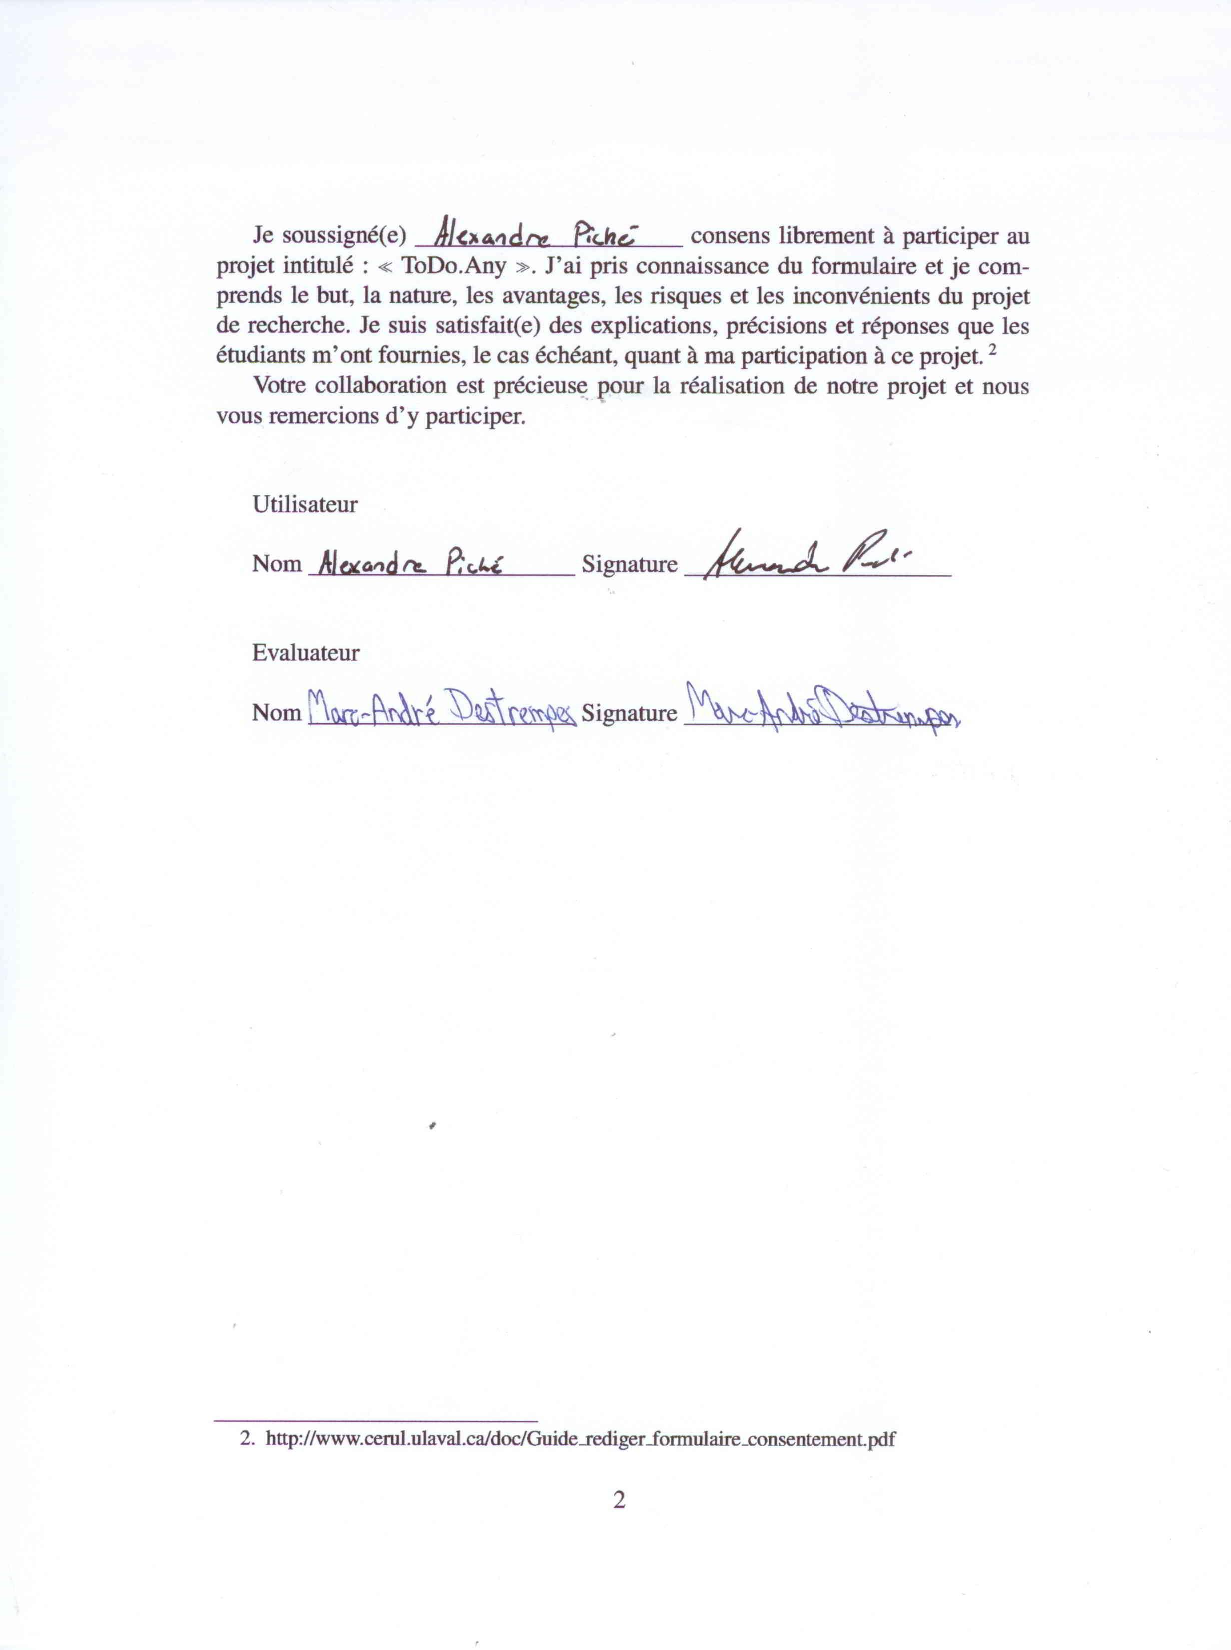
\includepdf[pages=-]{form_u1.pdf}
%
\includepdf[pages=-]{form_u0.pdf}
%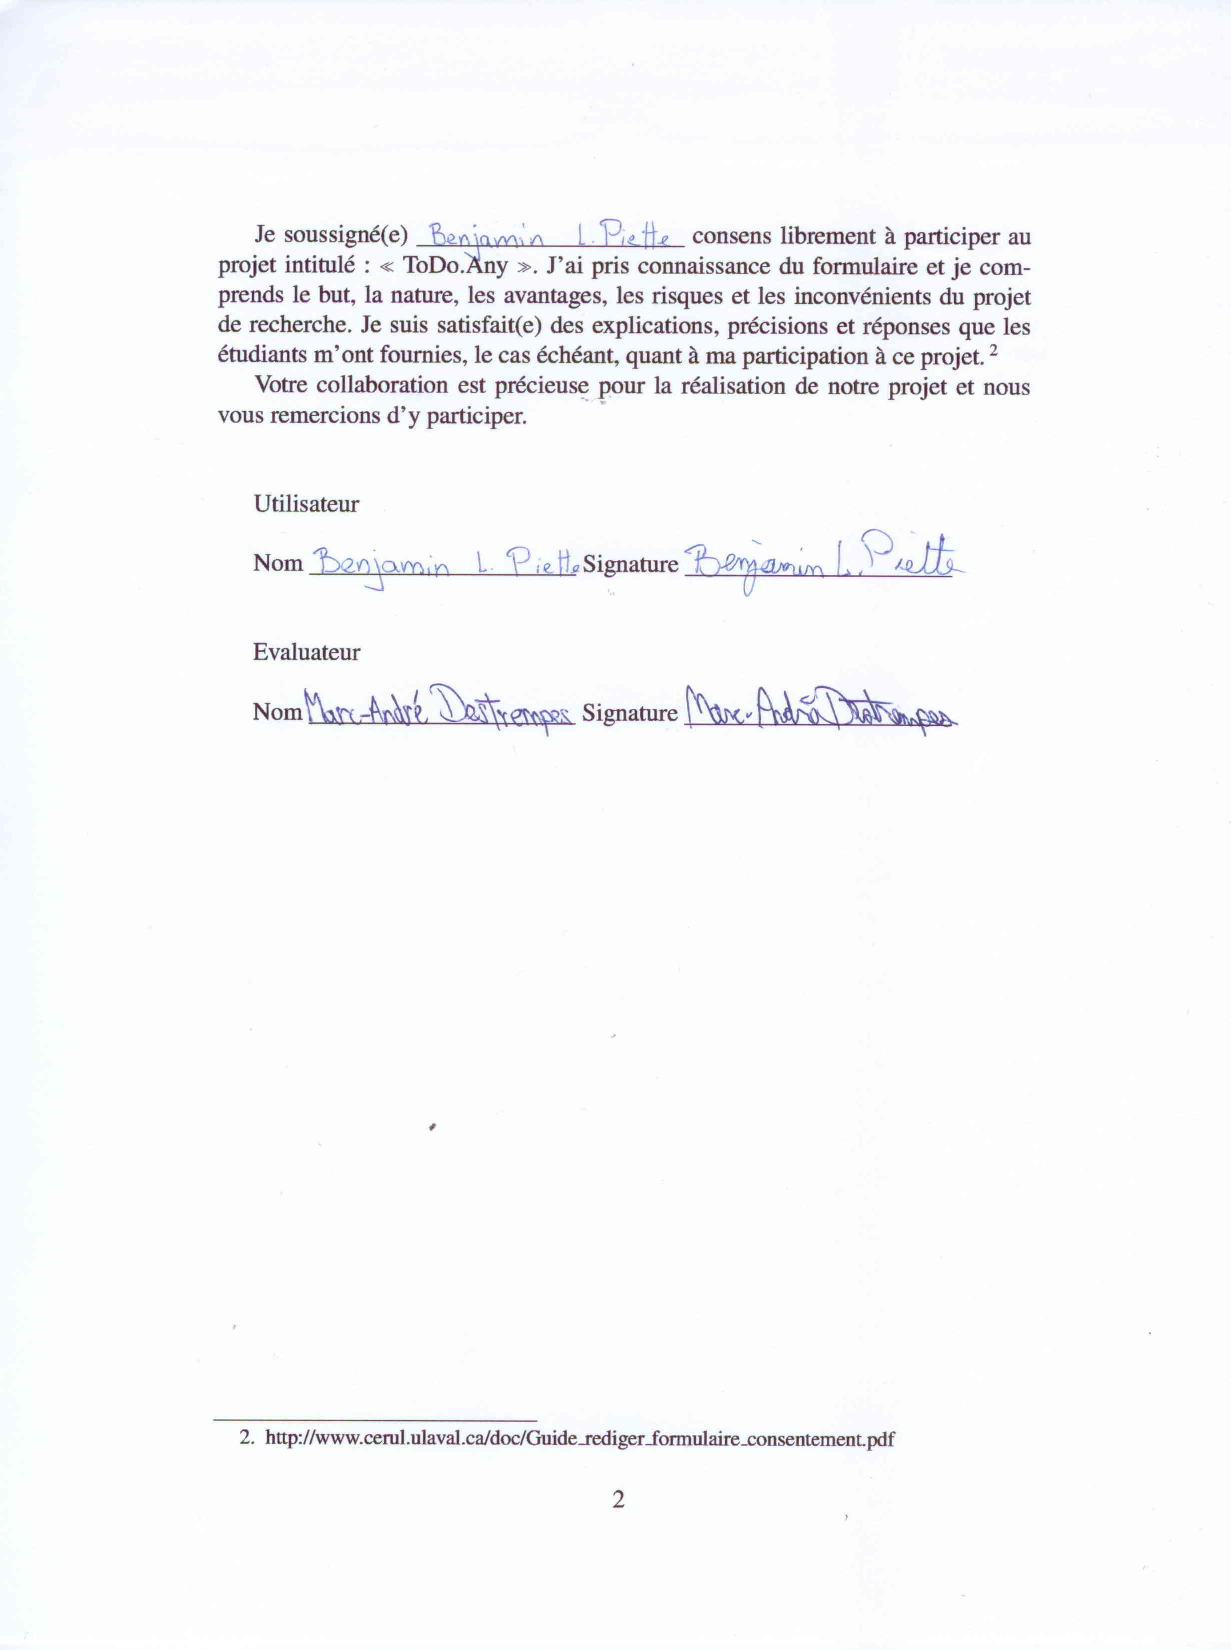
\includepdf[pages=-]{form_u2.pdf}

\chapter{Notes prises}

%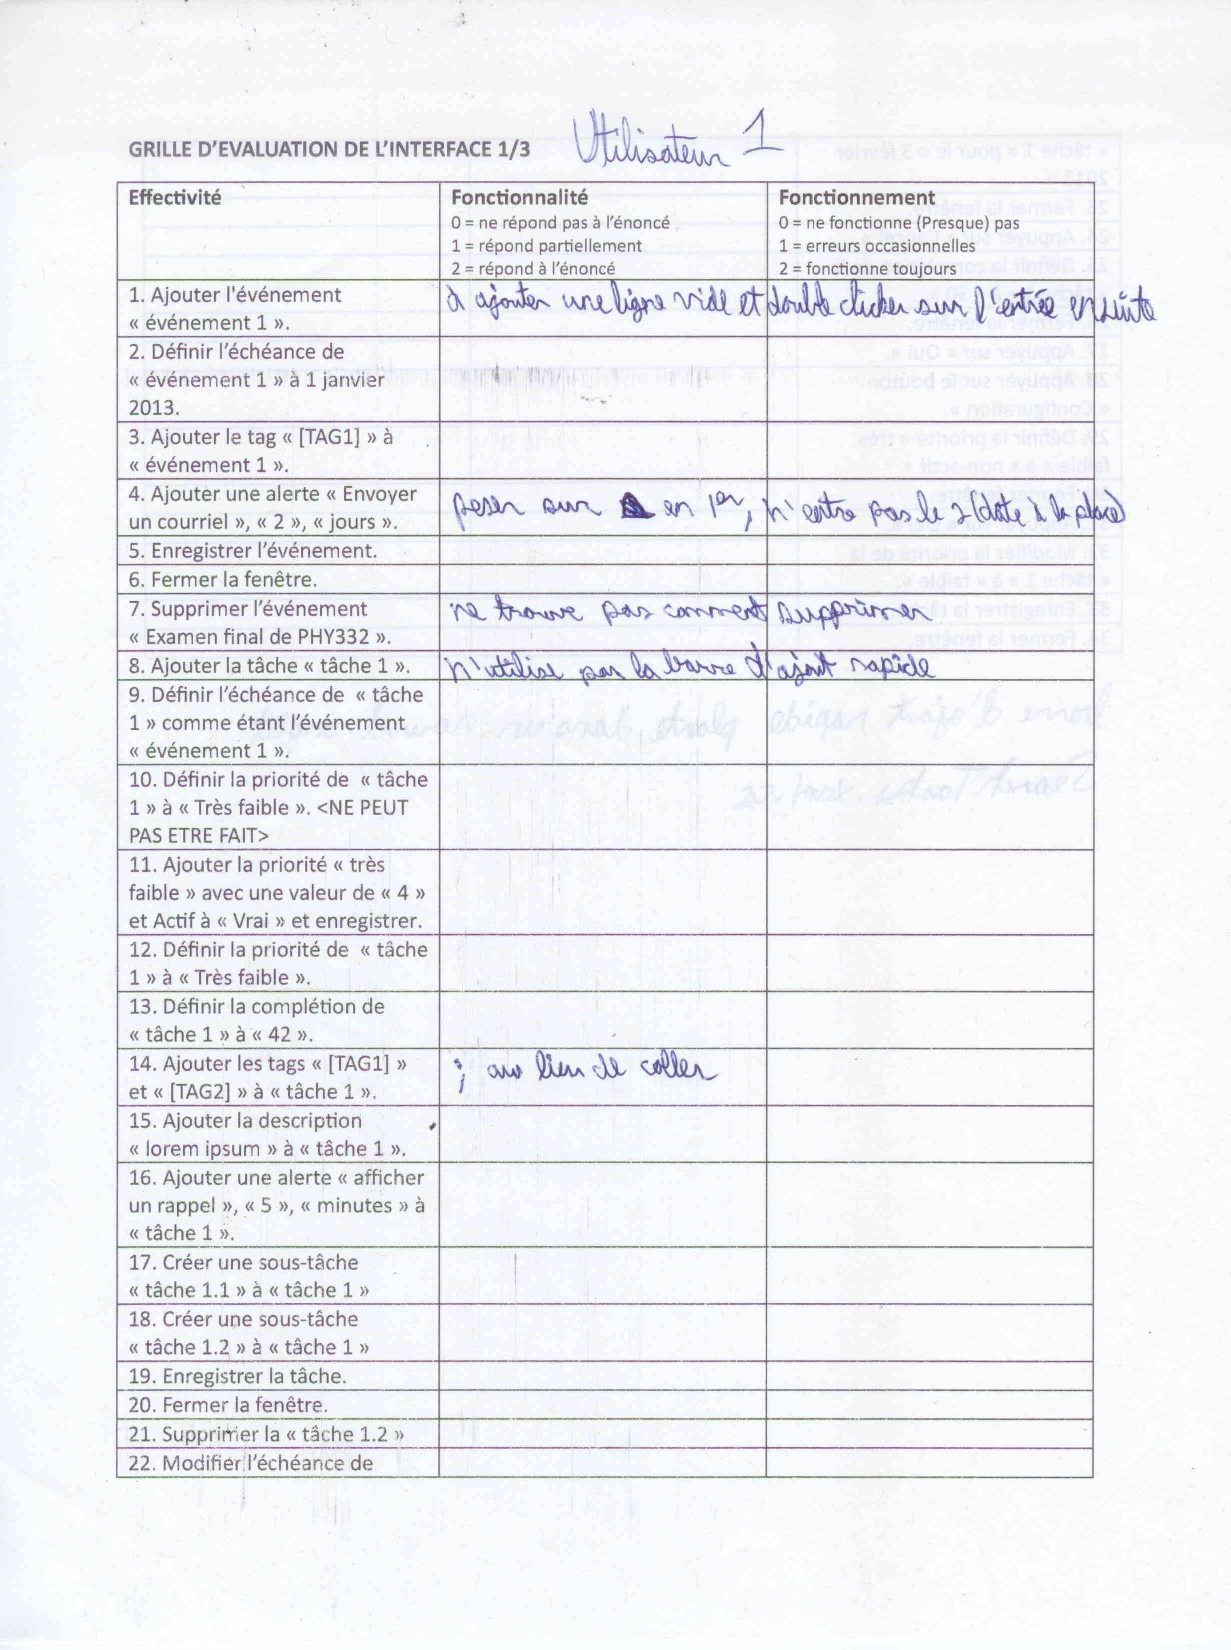
\includepdf[pages=-]{notes_p1.pdf}
%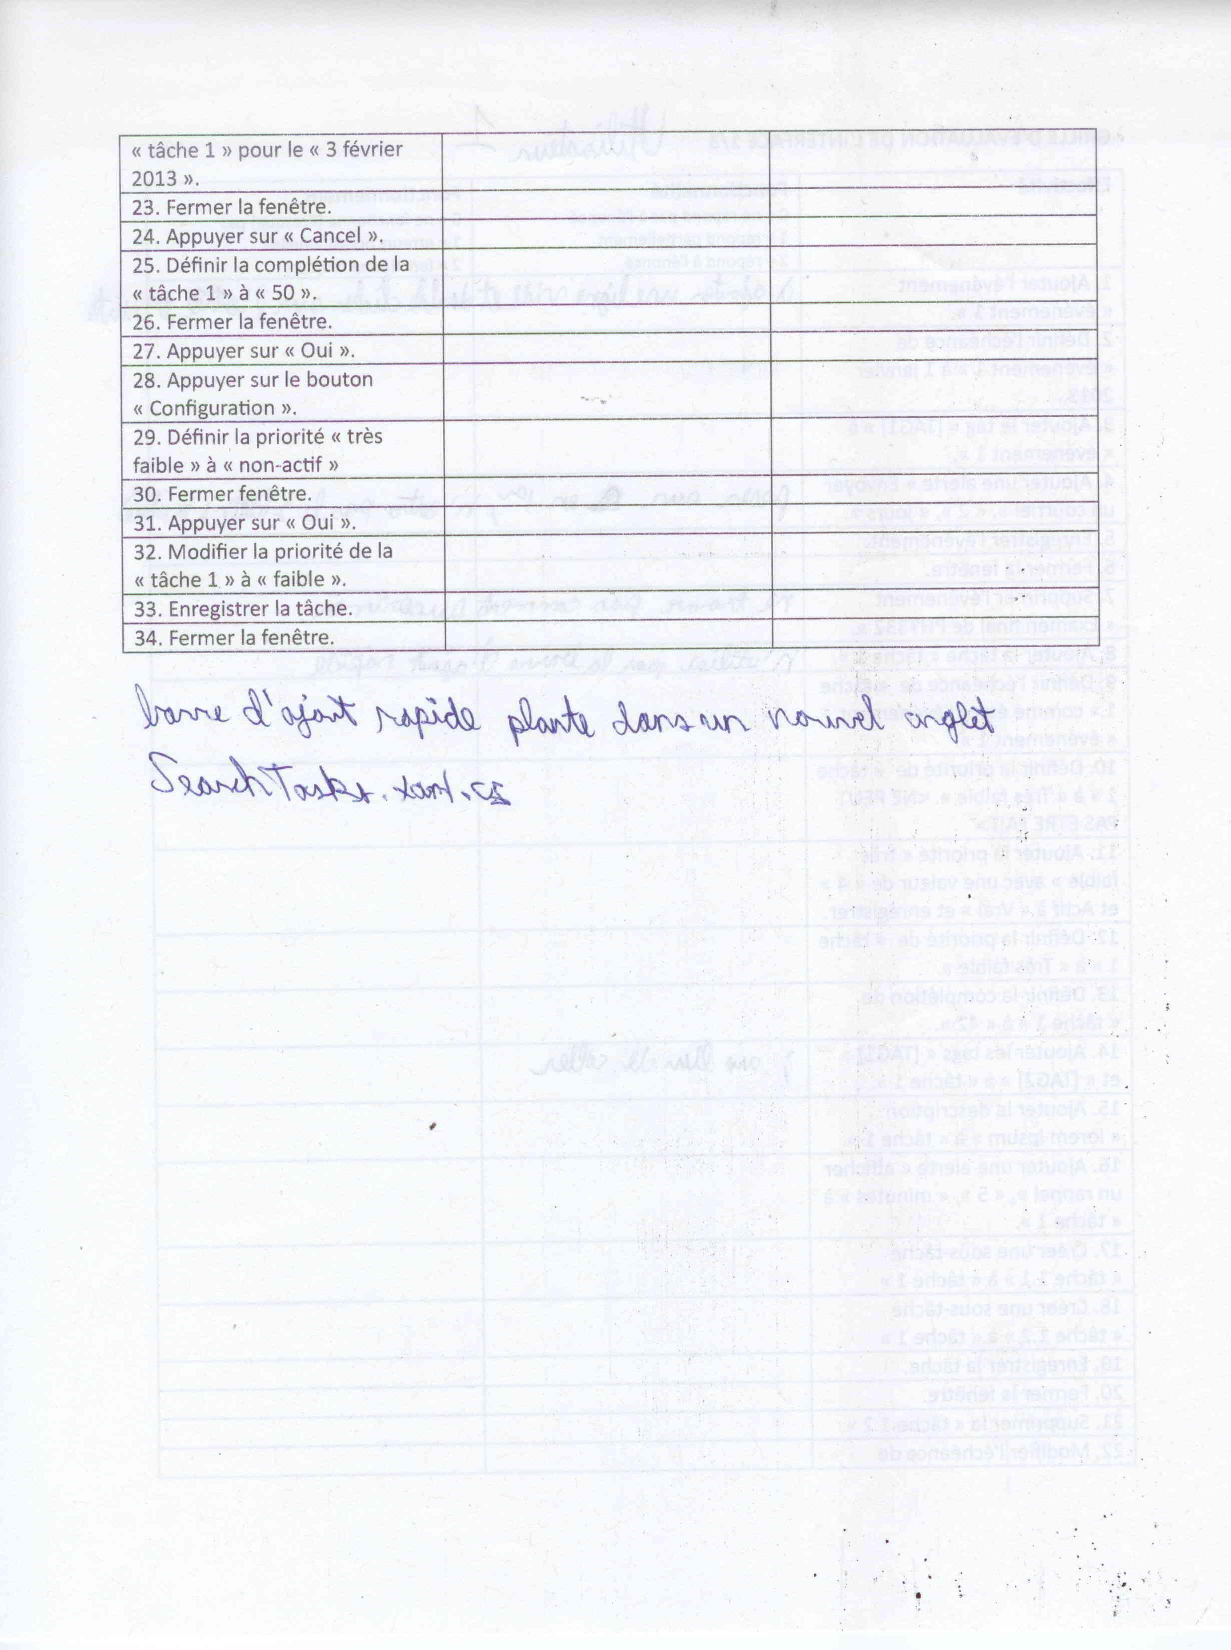
\includepdf[pages=-]{notes_p2.pdf}
%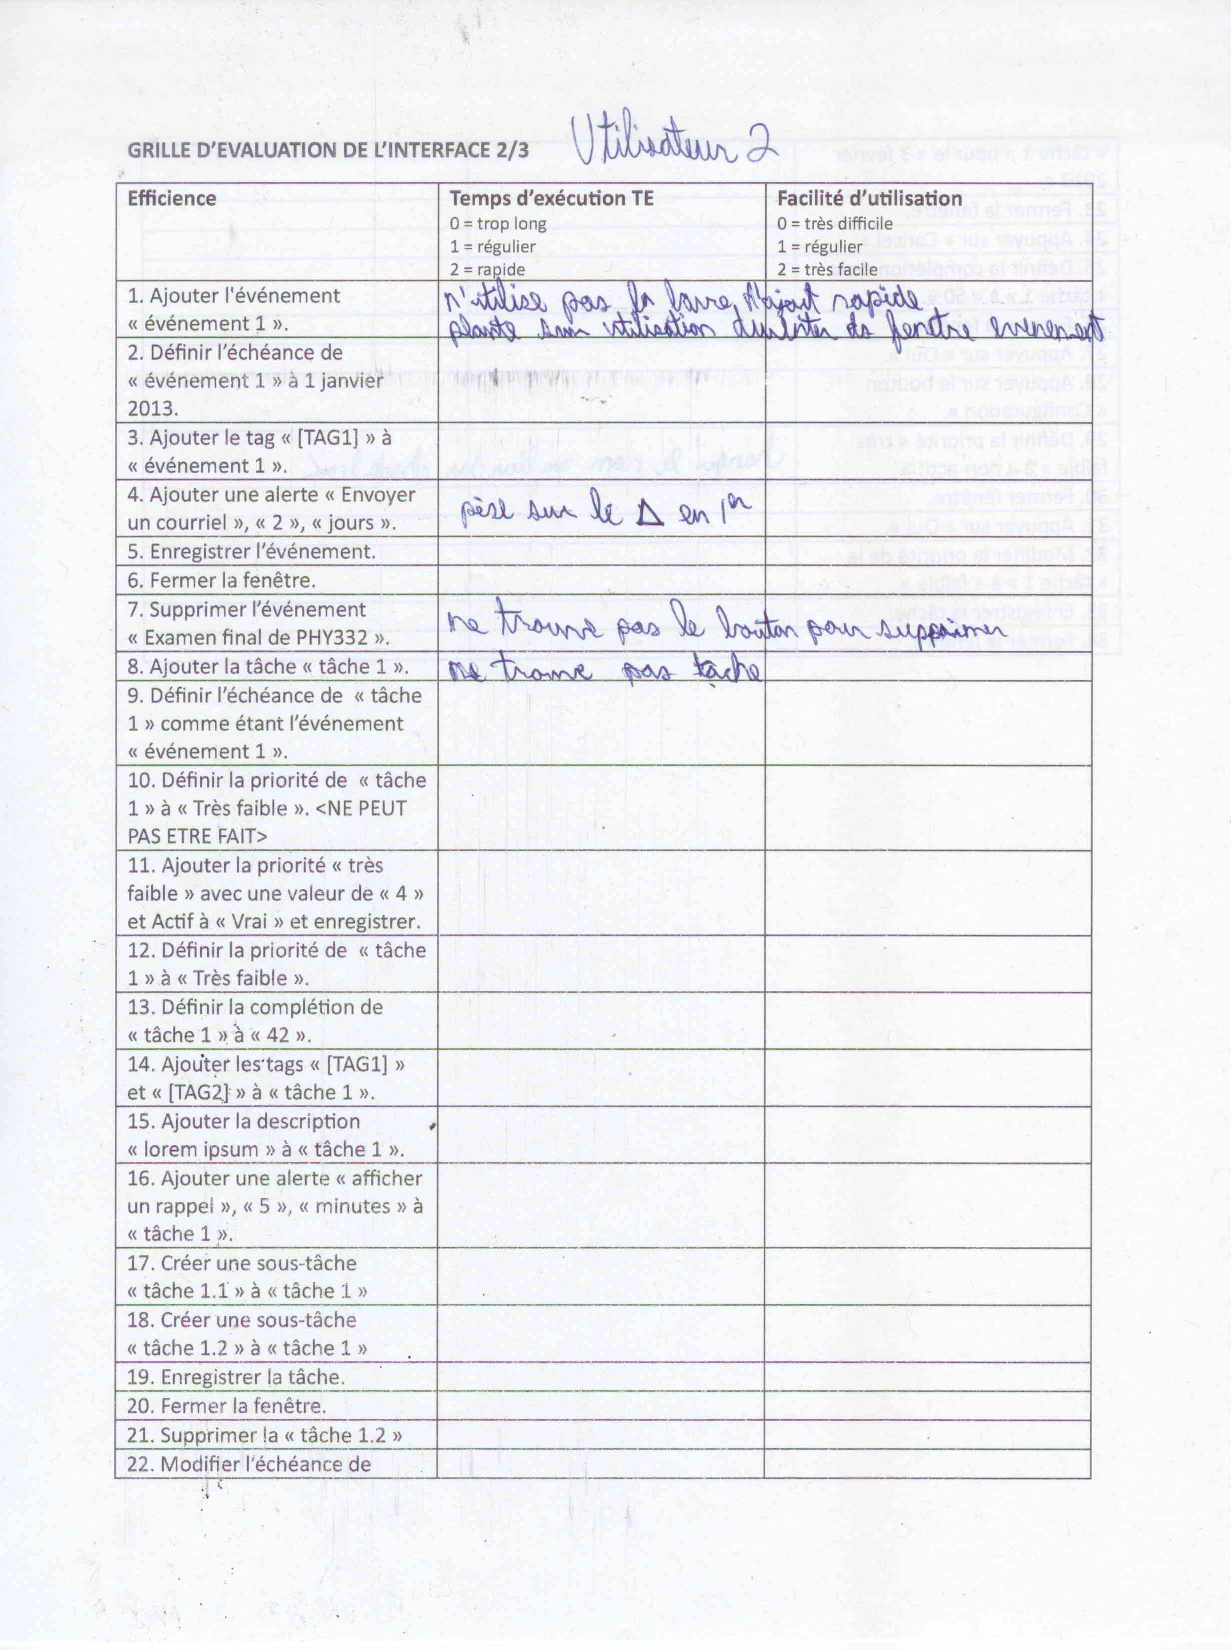
\includepdf[pages=-]{notes_p3.pdf}
%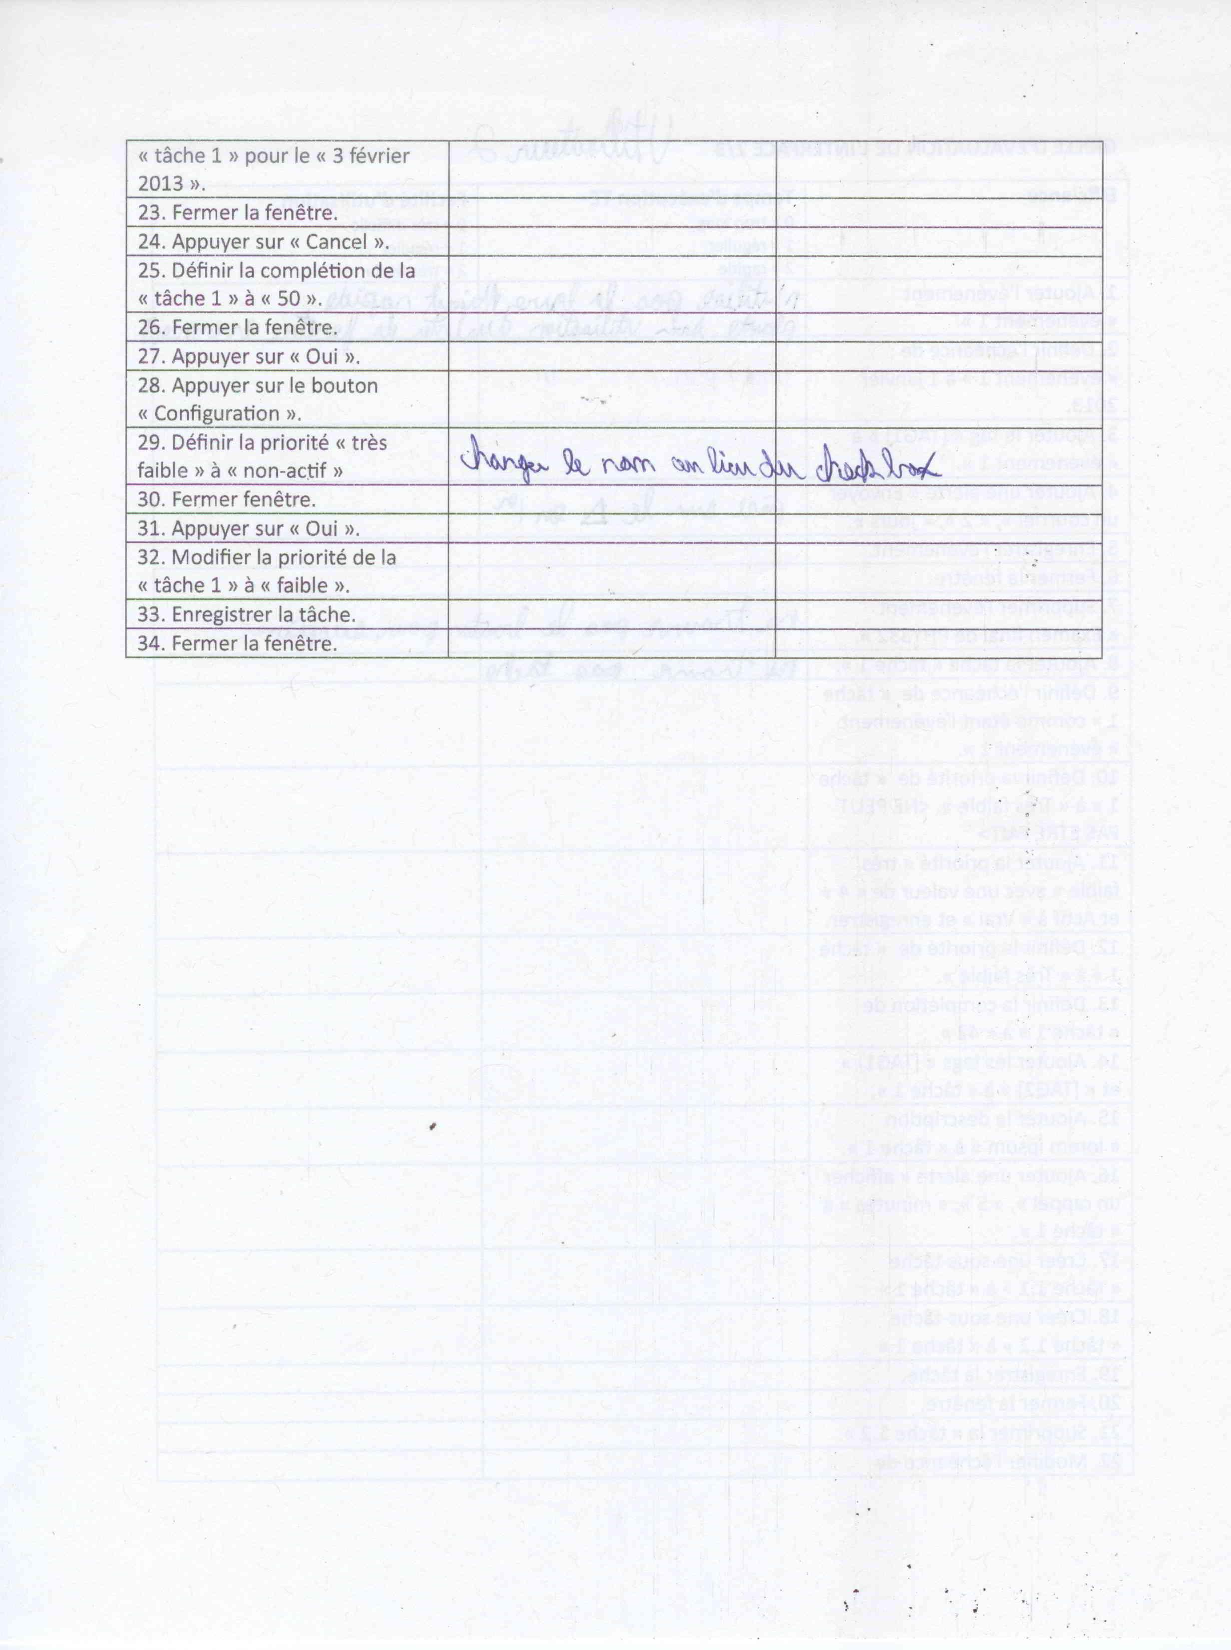
\includepdf[pages=-]{notes_p4.pdf}
%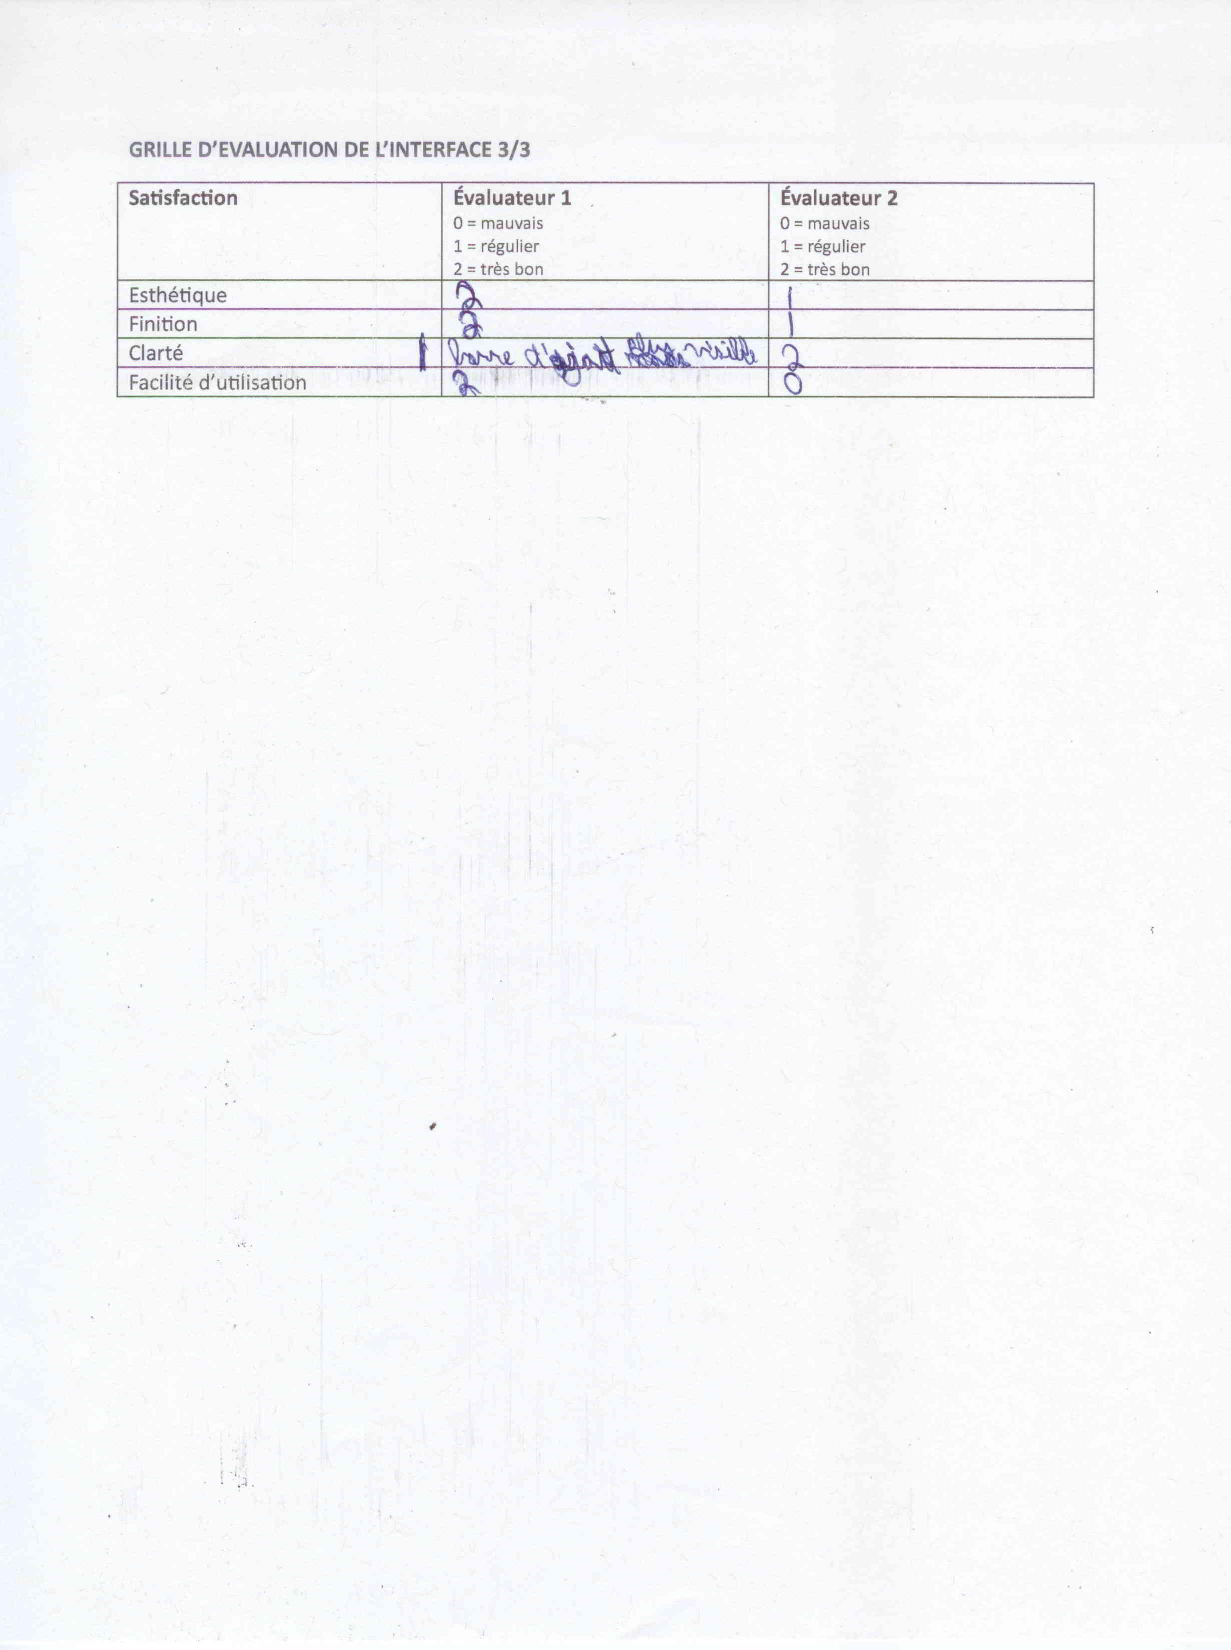
\includepdf[pages=-]{notes_p5.pdf}

\chapter{Travail Pratique 2}

%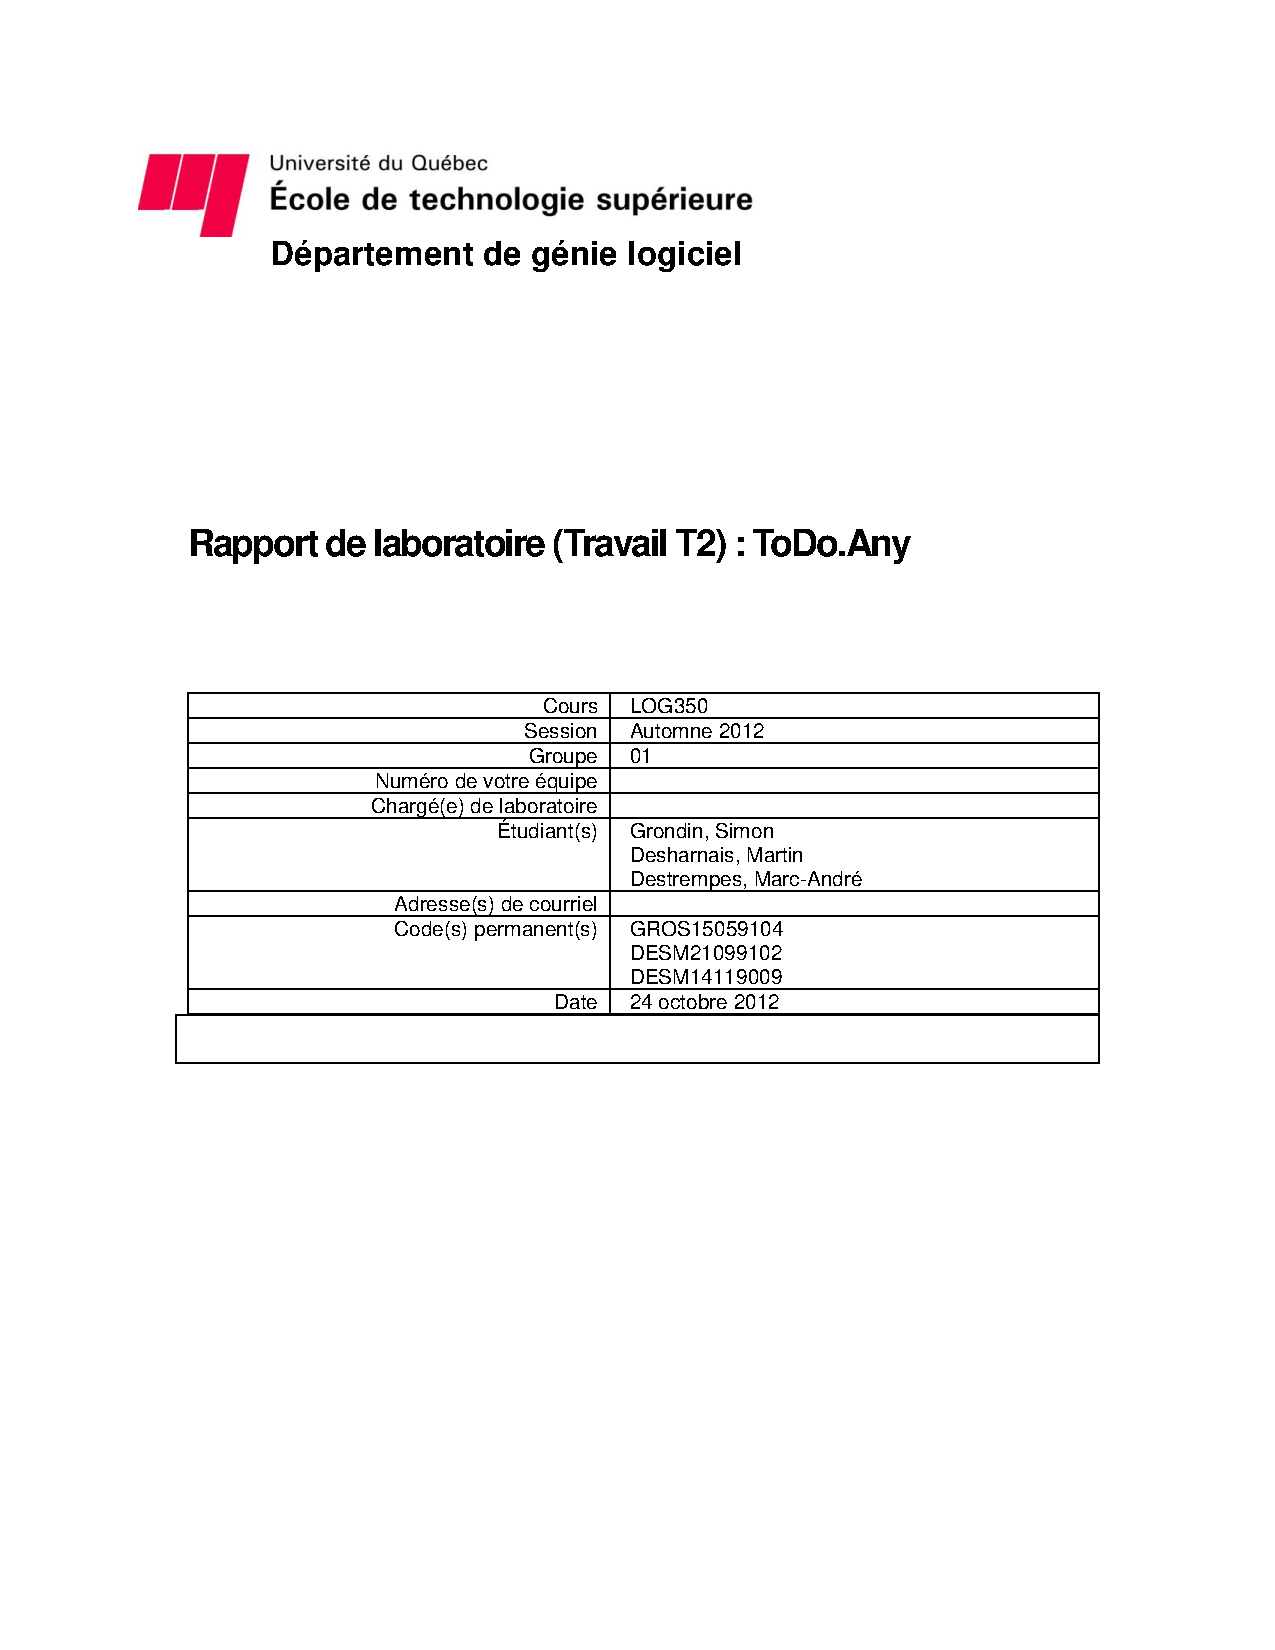
\includepdf[pages=-]{T2.pdf}


\end{document}
